\begin{table}[h!]
\centering
\begin{tabular}{|c|c|c|}
\hline
\textbf{Model name \& year} & \textbf{mAP}$_{50-95}$ & \textbf{Parameters (in Millions)} \\ \hline
YOLOv8n (2023)            & 37.3 & \textbf{3.2M} \\ \hline
YOLOv8m (2023)           & 50.2 & 25.9M \\ \hline
YOLOv8x (2023)            & \textbf{53.9} & 68.2M \\ \hline
Mask RCNN (2017)        & 34.9 & 63.7M \\ \hline
YOLOv3 (2018)            & 38.5 & 63.0M \\ \hline
\end{tabular}
\caption{Comparison of total model parameters (model size) and corresponding mean average precision (mAP) values obtained during training on the COCO dataset.}
\label{table:model-map-param}
\end{table}


%https://github.com/ultralytics/ultralytics#:~:text=TensorRT%0A(ms)-,params%0A(M),-FLOPs%0A(B)


In this paper, we endeavor to address the aforemetioned conundrums by establishing a comprehensive benchmarking framework that offers guidance to researchers in applying object detection within the realm of livestock production. Our investigation is centered around three pivotal questions:

\begin{enumerate} \label{contribution}
\item What methodologies ensure precise detection of various cattle breeds (Jersey, Holstein) in farm environments with differing lighting conditions and camera perspectives?
\item What is the minimum quantity of training samples required to attain a higher degree of accuracy?
\item Which model optimally balances the trade-off between detection accuracy and computational expenditure?
\end{enumerate}

To accomplish our objectives, we curated a diverse image dataset of dairy cattle, capturing a range of lighting conditions (daylight and nocturnal settings), camera angles (top-down and lateral views), and breeds (Holstein and Jersey). We evaluated the performance of state-of-the-art object detection frameworks, including YOLOv8, YOLONAS, YOLOv9 along with their varying model sizes, to discern their efficacy in detecting objects. In our analysis, we scrutinize the equilibrium between accuracy and computational demands to ascertain a model’s transferability. This benchmarking serves as a beacon for researchers aiming to implement object detection, providing a strategic approach to resource and effort allocation in their scholarly pursuits.





%%%%%%%%%%%%%%%%%%%%%%%%%
%%% Old problem Statement
\subsection{Contribution}

In this study, we present a systematic bench-marking study that addresses the concerns and provides a guidance for researchers, regardless of their expertise, to implement object detection in livestock production studies. Specifically, we aims to discuss three major perspectives of the implementation:
\begin{enumerate}
\item  How many training samples are required to achieve a certain accuracy?
\item  How much computational resources are required to implement the object detection?
\item  How much marginal efforts (i.e., samples) are required to transfer the model to a new environment?
\end{enumerate}
We will validate each goal by using state of the art object detection models, including YOLOv8, YOLONAS, Mask R-CNN, and transformer-based model DETR, with their variants that have different model sizes. For benchmarking the performance in tranferability, we collected image datasets of dairy cows and ensured the variation of the lighting environment (i.e., day and night), camera angles (i.e., top-down and side-view), and even the breeds (i.e., Holstein and Jersey). We will also discuss the trade-off between the accuracy and the computational resources. With this guidence, researchers who want to implemenet the object detection can have better management of their research resources and efforts.


\section{Problem Statements:}



\begin{enumerate}
    \item The task of determining the most suitable AI techniques for efficiently identifying and counting cows in the alley remains unsolved. While various AI models exist, from classification models that discern objects, detection models which undertake both classification and detection, to pose estimation models which pinpoint an object's pose, the question remains: which one is the most optimal for our specific application?

    \item A secondary concern relates to data optimization. With the multitude of available AI models, each differing in size and parameters (s, m, x being the key variants), it becomes imperative to ascertain the ideal number of images for training. The goal is to strike a balance between achieving high accuracy and ensuring reduced computational expenses.
    
    \item Lastly, How can we make the AI camera consistently detect and count cows  even with challenges like moving cows, different lighting, or blockages?
\end{enumerate}

In light of the aforementioned challenges, our research embarks on a quest for solutions:

\begin{enumerate}
    \item Through rigorous testing and evaluation, we have identified the object detection model as our chosen AI methodology, which will be further elucidated in the ensuing sections.

    \item Extensive training sessions, coupled with trials of varying data sample sizes and model dimensions, have led us to insightful conclusions. This research will expound on the ideal dataset size and model type that aligns with our goal of maximum accuracy and minimal computational demand.

    \item By emphasizing data diversity, we have sourced data from multiple perspectives and lighting conditions. Data derived from different cow breeds, including the likes of Jersey and Holstein, further enrich our dataset, ensuring our camera system's resilience against the wide array of challenges.
\end{enumerate}
By answering these questions, this research aims to bridge the gap between traditional alley management practices and cutting-edge AI solutions, offering a sustainable and efficient approach to dairy farming hygiene management.




%#####################
%% Added on 13/03/2024

Facebook's \textbf{DETR} (DEtection TRansformer) \cite{carion2020end} is a novel approach to object detection, diverging from the conventional region-based methods and moving towards a more end-to-end (a method that processes input data through all stages of computation to produce the final result within a single model or system) architecture. At its core, DETR employs the Transformer architecture\cite{vaswani2017attention}, which has previously been predominant in natural language processing tasks, particularly for its capability to handle sequences. In the context of DETR, this architecture processes the entire image as a sequence of flattened pixels. Unlike the traditional methods that rely on predicting anchor boxes, DETR treats object detection as a direct set prediction problem. Post the convolutional feature extraction, the model predicts a fixed number of bounding boxes and their respective class labels without any need for prior knowledge of the region proposals. This end-to-end approach simplifies the object detection pipeline by removing the intricacies of region proposal networks or anchor boxes, resulting in a more straightforward and intuitive methodology. Moreover, by leveraging the self-attention mechanism of Transformers, DETR can capture long-range dependencies and interactions between objects, making it especially effective in complex scenes.
%%%%%%%%%%%%% cross validation %%%%%%%%%%%%%%%%%%%%%
Cross-validation is a technique for determining how well a model will function on previously unknown data. We can consider it a method of testing a student's knowledge by splitting the study material into sections: while the student studies some parts, a few are kept hidden, only to be revealed during a surprise test. Similarly, in cross-validation, the data set is divided into "training" and "testing" sets many times. The model learns from the training set before being tested on an unknown testing set. This technique is repeated multiple (`k') times with different data divisions. We acquire a better sense of how well our model is going to perform in real-world circumstances by averaging the outcomes of these tests, ensuring that it isn't merely memorizing the data (or ``overfitting'') but is actually learning from it. Cross-validation, in essence, gives a more reliable measure of a model's performance and assures that it is ready for a variety of problems. Some of the major steps of the cross validation approach are described here.

\begin{enumerate}
    \item \textbf{Splitting the dataset}: Initially, the entire dataset is partitioned into 'k' subsets of approximately equal size. This division is done to prepare for a rotation of training and validation phases, where each subset gets a chance to play the role of the validation set.
    \item \textbf{Validation and training:} For each iteration or "fold":

    \begin{enumerate}
        \item One subset is designated as the validation set, and the rest are amalgamated to form the training set.
        \item The model is trained on the collective training set and then validated against the separate validation set. This ensures that the validation process is impartial and the model's predictions are tested on unseen data.
    \end{enumerate}

    \item \textbf{Repetition:} This process is repeated k times, with each k fold serving as the validation set just once.

    \item  \textbf{Average Performance:} After k rounds, you will have k various performance numbers (for example, accuracy, F1-score). Their average provides a more complete picture of the model's performance.
\end{enumerate}



%%%%%%021/03/2024
\subsection{YOLO Family Models}

In our endeavor to detect objects, we employed a selection of deep learning architectures, specifically: (1) YOLO V8 \cite{ultralyticsYOLOv8}, (2) YOLO V9 \cite{wang2024yolov9}, and (3) YOLO NAS \cite{ultralyticsYOLONASNeural}. The rationale behind opting for these particular models lies in their recency and their recognized state-of-the-art status. Importantly, most of the prior works in computer vision based object detection in either agriculture or animal science is done using Mask R CNN, or earlier version of the YOLO family Empirical evidence suggests that these architectures, in comparison to their predecessors, exhibit superior performance, both in terms of accuracy and latency, thereby making them suitable for our research objectives.

%\subsubsection{YOLO Family}
% why its called YOLO
YOLO has become a central real-time object detection system for agriculture, medicine and video monitoring applications. Within the vast field of object detection algorithms, the YOLO (You Only Look Once) framework has conspicuously emerged, distinguished by its adept synergy of processing speed and detection accuracy. Referring to the fact that it was able to accomplish the detection task with a single pass of the network, as opposed to previous approaches that either used sliding windows followed by a classifier that needed to run hundreds or thousands of times per image or the more advanced methods that divided the task into two-steps, where the first step detects possible regions with objects or regions proposals and the second step run a classifier on the proposals.

% different version of YOLO and Evolution
Tracing its lineage, the YOLO architecture has witnessed a series of evolutionary stages, spanning from its inaugural V1 version to YOLO V9. Each iteration represents a methodical advancement, refining upon its antecedents to mitigate limitations and augment performance. 

Initiated with YOLOv1 [cite], pioneered with its single-shot detection framework, markedly enhancing detection speeds by eliminating the need for separate proposal generation and refinement stages, thus enabling real-time performance. 

The advancement to YOLOv2[cite] and YOLOv3[cite] brought forward improvements in network architecture and training techniques. The introduction of batch normalization, which normalizes the inputs of each layer to reduce internal covariate shift, effectively made the model more stable. Anchor boxes were introduced to predict bounding boxes more accurately by pre-defining certain shapes and sizes that objects in the dataset commonly have. This method improved the detection of varying object sizes. Multi-scale training, another pivotal improvement, allowed the model to dynamically adjust the input size during training, making the network adept at detecting objects across different scales.

YOLOv4 [cite] marked further progression, incorporating mish activation, a smooth, non-monotonic function that facilitates the flow of gradients and helps in learning complex patterns more effectively. It also featured cross-stage partial connections (CSP), which split the feature map into two parts and then merged them through a cross-stage hierarchy, enhancing the learning capability while reducing computational cost. Self-adversarial training, a technique where the model is trained to generate adversarial examples itself, further refined the model's accuracy and robustness.

With YOLOv5, while unofficial in the sequence as it was developed by a different set of contributors, marked a significant step in making the technology more accessible and user-friendly. It focused on streamlining the model's architecture for better performance across a wide range of computing environments. A notable advancement in YOLOv5 is its utilization of PyTorch, enhancing the model's portability and ease of deployment. This version introduced adaptive anchor box calculations, improving the model's ability to detect objects of various sizes more accurately by dynamically adjusting anchor boxes based on dataset specifics. Additionally, YOLOv5 implemented automated batch size and image size adjustments, optimizing the training process to better utilize available hardware resources, thereby reducing training times without sacrificing accuracy.

YOLOv6 \cite{li2022yolov6} features a new backbone architecture called EfficientRep, which utilizes RepVGG's principles for higher parallelism, improving the model's ability to process images faster by doing more computations simultaneously. The neck of the model uses PAN (Path Aggregation Network) with RepBlocks or CSPStackRep Blocks, which help in efficiently combining features at different scales. An efficient decoupled head, inspired by YOLOX, optimizes the final object detection process. For better training outcomes, YOLOv6 adopts a task alignment learning approach for label assignment and introduces new loss functions: VariFocal loss for classification, enhancing the focus on more challenging examples, and SIoU/GIoU loss for regression, improving the precision of object localization. Additionally, a self-distillation strategy and a quantization scheme aid in making the model not only more accurate but also faster, with the largest model reaching $57.2\%$ AP on the MS COCO dataset at 29 FPS.

YOLOv7, on the other hand, introduces the Extended Efficient Layer Aggregation Network (E-ELAN), which allows for more efficient learning and convergence by managing the flow of gradients within unlimited stacked computational blocks. This approach helps in shuffling and merging features without compromising the original learning path, thereby enhancing the model's capability to learn from complex data. YOLOv7 also addresses the challenge of model scaling in concatenation-based architectures through a novel strategy that scales both the depth and width of blocks equally, ensuring optimal hardware utilization and maintaining the model's structure. Among the "bag of freebies," YOLOv7 utilizes Planned Re-parameterized Convolution (RepConvN) to avoid the residual and concatenation issues seen in previous versions. The model incorporates both coarse and fine label assignments for improved training efficiency, integrates batch normalization into convolution layers to streamline the inference process, draws on implicit knowledge inspired by YOLOR for enriched feature learning, and employs an exponential moving average for the final model, ensuring stability and robust performance.



Each iteration of the YOLO series not only outperformed its predecessors in terms of mean average precision (mAP) and frames per second (FPS) but also broadened the scope of real-world applications, showcasing the series' evolutionary strides in pushing the envelope of computer vision technology. YOLOv8, and YOLOv9 is the latest models from the YOLO family. And in our work we primarily focused on these models.




\subsection{YOLO Family Models}



%\subsubsection{YOLO Family}
% different version of YOLO and Evolution
Tracing its lineage, the YOLO architecture has witnessed a series of evolutionary stages, spanning from its V1 version to YOLO V9. Each iteration represents a methodical advancement, refining upon its antecedents to mitigate limitations and augment performance. 
% why its called YOLO
YOLO has become a central real-time object detection system for agriculture, medicine and video monitoring applications. Within the vast field of object detection algorithms, the YOLO (You Only Look Once) framework has conspicuously emerged, distinguished by its adept synergy of processing speed and detection accuracy. Initiated with YOLOv1 \cite{redmon2016you}, pioneered with its single-shot detection framework, markedly enhancing detection speeds by eliminating the need for separate proposal generation and refinement stages, thus enabling real-time performance. Referring to the fact that it was able to accomplish the detection task with a single pass of the network, as opposed to previous approaches that either used sliding windows followed by a classifier that needed to run hundreds or thousands of times per image or the more advanced methods that divided the task into two-steps, where the first step detects possible regions with objects or regions proposals and the second step run a classifier on the proposals.


The advancement to YOLOv2 \cite{redmon2017yolo9000} and YOLOv3 \cite{redmon2018yolov3} brought forward improvements in network architecture and training techniques. The introduction of batch normalization, which normalizes the inputs of each layer to reduce internal covariate shift, effectively made the model more stable. Anchor boxes were introduced to predict bounding boxes more accurately by pre-defining certain shapes and sizes that objects in the dataset commonly have. This method improved the detection of varying object sizes. Multi-scale training, another pivotal improvement, allowed the model to dynamically adjust the input size during training, making the network adept at detecting objects across different scales.

YOLOv4 \cite{bochkovskiy2020yolov4} marked further progression, incorporating mish activation, a smooth, non-monotonic function that facilitates the flow of gradients and helps in learning complex patterns more effectively. It also featured cross-stage partial connections (CSP), which split the feature map into two parts and then merged them through a cross-stage hierarchy, enhancing the learning capability while reducing computational cost. Self-adversarial training, a technique where the model is trained to generate adversarial examples itself, further refined the model's accuracy and robustness.

With YOLOv5 \cite{Jocher2020YOLOv5}, while unofficial in the sequence as it was developed by a different set of contributors, marked a significant step in making the technology more accessible and user-friendly. It focused on streamlining the model's architecture for better performance across a wide range of computing environments. A notable advancement in YOLOv5 is its utilization of PyTorch, enhancing the model's portability and ease of deployment. This version introduced adaptive anchor box calculations, improving the model's ability to detect objects of various sizes more accurately by dynamically adjusting anchor boxes based on dataset specifics. Additionally, YOLOv5 implemented automated batch size and image size adjustments, optimizing the training process to better utilize available hardware resources, thereby reducing training times without sacrificing accuracy.

YOLOv6 \cite{li2022yolov6} features a new backbone architecture called EfficientRep, improving the model's ability to process images faster by doing more computations simultaneously. Additionally, a self-distillation strategy and a quantization scheme aid in making the model not only more accurate but also faster, with the largest model reaching $57.2\%$ AP on the MS COCO dataset at 29 FPS.

YOLOv7 \cite{wang2023yolov7}, on the other hand, introduces the Extended Efficient Layer Aggregation Network (E-ELAN), which allows for more efficient learning and convergence by managing the flow of gradients within unlimited stacked computational blocks. This approach helps in shuffling and merging features without compromising the original learning path, thereby enhancing the model's capability to learn from complex data. YOLOv7 also addresses the challenge of model scaling in concatenation-based architectures through a novel strategy that scales both the depth and width of blocks equally, ensuring optimal hardware utilization and maintaining the model's structure. 


Each iteration of the YOLO series not only outperformed its predecessors in terms of mean average precision (mAP) and frames per second (FPS) but also broadened the scope of real-world applications, showcasing the series' evolutionary strides in pushing the envelope of computer vision technology. YOLOv8, and YOLOv9 is the latest models from the YOLO family. And in our work we primarily focused on these models.


%\subsubsection*{YOLO V8}
%\paragraph{YOLO V8:}

\textbf{YOLOv8} \cite{ultralyticsYOLOv8} YOLOv8 represents a significant advancement in the YOLO series of object detection models, offering several improvements over its predecessors. It retains a similar backbone to YOLOv5, but introduces the C2f module, enhancing feature integration for better detection accuracy. This new module allows for the effective combination of high-level features with contextual information, which is particularly beneficial for detecting objects with precision.

A notable change in YOLOv8 is the transition to an anchor-free model with a decoupled head, which processes the tasks of objectness, classification, and regression separately. This specialized approach enables each branch of the model to concentrate on its respective task, improving overall accuracy. In the output layer, YOLOv8 employs the sigmoid activation function for object presence in bounding boxes and the softmax function for class probabilities, optimizing the probability representations for each object class.

For loss functions, YOLOv8 utilizes CIoU and DFL loss functions for bounding-box accuracy, enhancing the model's performance with small objects, and binary cross-entropy for classification loss. These improvements contribute to the model's proficiency in object detection tasks.

Additionally, YOLOv8 extends its capabilities beyond object detection by including a semantic segmentation model, YOLOv8-Seg. This model employs the same CSPDarknet53 backbone followed by the C2f module, diverging from the traditional YOLO neck architecture. The model features two segmentation heads designed to predict semantic segmentation masks, further enhancing the model's utility.




%Drawback of Yolo v8 which has overcomed in v9......
One  drawback of deep learning modes is that they suffer some degree of information bottleneck [cite]. In general words, information bottleneck refers to the phenomenon of how well feature-map can retain information of its previous layers or even input image. When you have a large amount of data or information, in this case input image, and we need to compress it or summarize in form of features, there will be information loss. On the other hand, information bottleneck specifically refers to the challenge of reducing the amount of information processed by a network to the minimum necessary to perform a task without losing significant detail that would degrade the network's performance. This is like making sure that even though the canyon is narrow, the most important traffic (essential information) gets through efficiently. In general, as we go deeper in the feed forward process, the gradient loos becomes inevitable. One way to solve this increase the width of the model. When we use more parameters in the model, even if the information is lost during data feed forward process there is still achangce to retain enogh informtation to perform the feature mapping. 

However, this does not fundamentally changes the problem of information loss. As the networks size increases and layers go deeper, the model tendency to suffer from generating more unreliable gradients. We can compare this to garbage information. This is why even we increase the size of the parameters significantly, we may not see the significant imporovement of the result. Even in somecase, where there is single class, the model with larger parameters may perform not any better than models with smaller number of paramter.

To overcome this issue, many methods are used such as ResNET, versions of CSPNet,ELAN etc in different versions of YOLO. However, YOLOv9 \cite{wang2024yolov9} heavily improvised the existing methods. YOLOv9 incorporates Programmable Gradient Information (PGI) and the Generalized Efficient Layer Aggregation Network (GELAN). PGI is a technique that enhances the generation of reliable gradients during the training of the model, which is particularly useful for combating information loss across deep network layers. GELAN, on the other hand, is a flexible architecture that allows the integration of various computational blocks, optimizing the network for efficient resource usage and scalable object detection.


In terms of performance, YOLOv9 demonstrates superior results on the MS COCO dataset for object detection, outperforming previous models in terms of parameter utilization and achieving better results than state-of-the-art models pre-trained using large datasets. The architecture employs conventional convolution operators, which are shown to be more effective than the depth-wise convolution utilized in some of the latest methods.

%3################### Beside these, x, world, 3d,
Beside these yolo versions yolo has also some other models like YOLOX, YOLOR, YOLO-NAS, YOLO world etc. 







% Yolo Nas
alongside YOLO-NAS (Neural Architecture Search), epitomizes this journey, employing cutting-edge machine learning techniques to redefine benchmarks for real-time object detection systems. The consistent enhancement in performance metrics across versions highlights the series' dedication to refining the efficacy and efficiency of object detection methodologies (Terven, Córdova-Esparza, $\&$ Romero-González, 2023).




%\subsubsection*{YOLO NAS}
\textbf{YOLO-NAS} \cite{ultralyticsYOLONASNeural} was released in May 2023 by Deci, a company that develops production-grade models and tools to
build, optimize, and deploy deep learning models. YOLO-NAS is designed to detect small objects, improve localization
accuracy, and enhance the performance-per-compute ratio, making it suitable for real-time edge-device applications. YOLO-NAS models have been released in FP32, FP16, and INT8 precisions, achieving an AP of
$52.2\%$ on MS COCO with 16-bit precision 
\cite{terven2304comprehensive}.




In our endeavor to detect objects, we employed a selection of deep learning architectures, specifically: (1) YOLO V8 \cite{ultralyticsYOLOv8}, (2) YOLO V9 \cite{wang2024yolov9}, and (3) YOLO NAS \cite{ultralyticsYOLONASNeural}. The rationale behind opting for these particular models lies in their recency and their recognized state-of-the-art status. Importantly, most of the prior works in computer vision based object detection in either agriculture or animal science is done using Mask R CNN, or earlier version of the YOLO family Empirical evidence suggests that these architectures, in comparison to their predecessors, exhibit superior performance, both in terms of accuracy and latency, thereby making them suitable for our research objectives.


- YOLO structure
- YOLOv8
- YOLONAS
- YOLOv9




%############ 03/22/2024

\subsection{YOLO Family Models}



%\subsubsection{YOLO Family}
% different version of YOLO and Evolution
Tracing its lineage, the YOLO architecture has witnessed a series of evolutionary stages, spanning from its versions YOLO V1 to YOLO V9 along with some other variants. Each iteration represents a methodical advancement, refining upon its antecedents to mitigate limitations and augment performance. 


% why its called YOLO
YOLO models has become a central real-time object detection system for agriculture, medicine and video monitoring applications. Within the vast field of object detection algorithms, the YOLO (You Only Look Once) framework has conspicuously emerged, distinguished by its adept synergy of processing speed and detection accuracy. Tracing its lineage, the YOLO architecture has witnessed a series of evolutionary stages, spanning from its versions YOLO V1 to YOLO V9 along with some other variants.

Initiated with YOLOv1 \cite{redmon2016you}, pioneered with its single-shot detection framework, markedly enhancing detection speeds by eliminating the need for separate proposal generation and refinement stages, thus enabling real-time performance. Referring to the fact that it was able to accomplish the detection task with a single pass of the network, as opposed to previous approaches that either used sliding windows followed by a classifier that needed to run hundreds or thousands of times per image or the more advanced methods that divided the task into two-steps, where the first step detects possible regions with objects or regions proposals and the second step run a classifier on the proposals.


The advancement to YOLOv2 \cite{redmon2017yolo9000} and YOLOv3 \cite{redmon2018yolov3} brought forward improvements in network architecture and training techniques. The introduction of batch normalization, which normalizes the inputs of each layer to reduce internal covariate shift, effectively made the model more stable. 

YOLOv4 \cite{bochkovskiy2020yolov4} marked further progression, incorporating mish activation, a smooth, non-monotonic function that facilitates the flow of gradients and helps in learning complex patterns more effectively. It also featured cross-stage partial connections (CSP), which split the feature map into two parts and then merged them through a cross-stage hierarchy, enhancing the learning capability while reducing computational cost. Self-adversarial training, a technique where the model is trained to generate adversarial examples itself, further refined the model's accuracy and robustness.

With YOLOv5 \cite{Jocher2020YOLOv5}, marked a significant step in making the technology more accessible and user-friendly. It focused on streamlining the model's architecture for better performance across a wide range of computing environments. A notable advancement in YOLOv5 is its utilization of PyTorch, enhancing the model's portability and ease of deployment. This version introduced adaptive anchor box calculations, improving the model's ability to detect objects of various sizes more accurately by dynamically adjusting anchor boxes based on dataset specifics. Additionally, YOLOv5 implemented automated batch size and image size adjustments, optimizing the training process to better utilize available hardware resources, thereby reducing training times without sacrificing accuracy.

YOLOv6 \cite{li2022yolov6} features a new backbone architecture called EfficientRep, improving the model's ability to process images faster by doing more computations simultaneously. Additionally, a self-distillation strategy and a quantization scheme aid in making the model not only more accurate but also faster, with the largest model reaching $57.2\%$ AP on the MS COCO dataset at 29 FPS.

YOLOv7 \cite{wang2023yolov7}, on the other hand, introduces the Extended Efficient Layer Aggregation Network (E-ELAN), which allows for more efficient learning and convergence by managing the flow of gradients within unlimited stacked computational blocks. This approach helps in shuffling and merging features without compromising the original learning path, thereby enhancing the model's capability to learn from complex data. YOLOv7 also addresses the challenge of model scaling in concatenation-based architectures through a novel strategy that scales both the depth and width of blocks equally, ensuring optimal hardware utilization and maintaining the model's structure. 


Each iteration of the YOLO series not only outperformed its predecessors in terms of mean average precision (mAP) and frames per second (FPS) but also broadened the scope of real-world applications, showcasing the series' evolutionary strides in pushing the envelope of computer vision technology. YOLOv8, and YOLOv9 is the latest models from the YOLO family. And in our work we primarily focused on these models.


%\subsubsection*{YOLO V8}
%\paragraph{YOLO V8:}

\textbf{YOLOv8} \cite{ultralyticsYOLOv8} YOLOv8 represents a significant advancement in the YOLO series of object detection models, offering several improvements over its predecessors. It retains a similar backbone to YOLOv5, but introduces the C2f module, enhancing feature integration for better detection accuracy. This new module allows for the effective combination of high-level features with contextual information, which is particularly beneficial for detecting objects with precision.

A notable change in YOLOv8 is the transition to an anchor-free model with a decoupled head, which processes the tasks of objectness, classification, and regression separately. This specialized approach enables each branch of the model to concentrate on its respective task, improving overall accuracy. In the output layer, YOLOv8 employs the sigmoid activation function for object presence in bounding boxes and the softmax function for class probabilities, optimizing the probability representations for each object class.

For loss functions, YOLOv8 utilizes CIoU and DFL loss functions for bounding-box accuracy, enhancing the model's performance with small objects, and binary cross-entropy for classification loss. These improvements contribute to the model's proficiency in object detection tasks.

Additionally, YOLOv8 extends its capabilities beyond object detection by including a semantic segmentation model, YOLOv8-Seg. This model employs the same CSPDarknet53 backbone followed by the C2f module, diverging from the traditional YOLO neck architecture. The model features two segmentation heads designed to predict semantic segmentation masks, further enhancing the model's utility.




%Drawback of Yolo v8 which has overcomed in v9......
One  drawback of deep learning modes is that they suffer some degree of information bottleneck [cite]. In general words, information bottleneck refers to the phenomenon of how well feature-map can retain information of its previous layers or even input image. When you have a large amount of data or information, in this case input image, and we need to compress it or summarize in form of features, there will be information loss. On the other hand, information bottleneck specifically refers to the challenge of reducing the amount of information processed by a network to the minimum necessary to perform a task without losing significant detail that would degrade the network's performance. This is like making sure that even though the canyon is narrow, the most important traffic (essential information) gets through efficiently. In general, as we go deeper in the feed forward process, the gradient loos becomes inevitable. One way to solve this increase the width of the model. When we use more parameters in the model, even if the information is lost during data feed forward process there is still achangce to retain enogh informtation to perform the feature mapping. 

However, this does not fundamentally changes the problem of information loss. As the networks size increases and layers go deeper, the model tendency to suffer from generating more unreliable gradients. We can compare this to garbage information. This is why even we increase the size of the parameters significantly, we may not see the significant imporovement of the result. Even in somecase, where there is single class, the model with larger parameters may perform not any better than models with smaller number of paramter.

To overcome this issue, many methods are used such as ResNET, versions of CSPNet,ELAN etc in different versions of YOLO. However, YOLOv9 \cite{wang2024yolov9} heavily improvised the existing methods. YOLOv9 incorporates Programmable Gradient Information (PGI) and the Generalized Efficient Layer Aggregation Network (GELAN). PGI is a technique that enhances the generation of reliable gradients during the training of the model, which is particularly useful for combating information loss across deep network layers. GELAN, on the other hand, is a flexible architecture that allows the integration of various computational blocks, optimizing the network for efficient resource usage and scalable object detection.


In terms of performance, YOLOv9 demonstrates superior results on the MS COCO dataset for object detection, outperforming previous models in terms of parameter utilization and achieving better results than state-of-the-art models pre-trained using large datasets. The architecture employs conventional convolution operators, which are shown to be more effective than the depth-wise convolution utilized in some of the latest methods.

%3################### Beside these, x, world, 3d,
Beside these yolo versions yolo has also some other models like YOLOX, YOLOR, YOLO-NAS, YOLO world etc. 







% Yolo Nas
alongside YOLO-NAS (Neural Architecture Search), epitomizes this journey, employing cutting-edge machine learning techniques to redefine benchmarks for real-time object detection systems. The consistent enhancement in performance metrics across versions highlights the series' dedication to refining the efficacy and efficiency of object detection methodologies (Terven, Córdova-Esparza, $\&$ Romero-González, 2023).




%\subsubsection*{YOLO NAS}
\textbf{YOLO-NAS} \cite{ultralyticsYOLONASNeural} was released in May 2023 by Deci, a company that develops production-grade models and tools to
build, optimize, and deploy deep learning models. YOLO-NAS is designed to detect small objects, improve localization
accuracy, and enhance the performance-per-compute ratio, making it suitable for real-time edge-device applications. YOLO-NAS models have been released in FP32, FP16, and INT8 precisions, achieving an AP of
$52.2\%$ on MS COCO with 16-bit precision 
\cite{terven2304comprehensive}.




In our endeavor to detect objects, we employed a selection of deep learning architectures, specifically: (1) YOLO V8 \cite{ultralyticsYOLOv8}, (2) YOLO V9 \cite{wang2024yolov9}, and (3) YOLO NAS \cite{ultralyticsYOLONASNeural}. The rationale behind opting for these particular models lies in their recency and their recognized state-of-the-art status. Importantly, most of the prior works in computer vision based object detection in either agriculture or animal science is done using Mask R CNN, or earlier version of the YOLO family Empirical evidence suggests that these architectures, in comparison to their predecessors, exhibit superior performance, both in terms of accuracy and latency, thereby making them suitable for our research objectives.


- YOLO structure
- YOLOv8
- YOLONAS
- YOLOv9



%%% Old version of YOLO family models
\subsection{YOLO Family Models}


YOLO models have gained popularity in real time object detection applications, across fields like agriculture, medicine and video monitoring. Among the array of object detection algorithms the YOLO (You Look Once) framework stands out for its effective balance of speed and accuracy in detection. Evolving through versions from YOLO V1 to YOLO V9 and variants, like YOLO NAS, YOLO World etc. Each iteration represents a systematic improvement building upon its predecessors to address limitations and enhance performance.


YOLOv8 \cite{ultralyticsYOLOv8} marks a step, in the YOLO series of object detection models bringing several enhancements compared to its predecessors. While maintaining a foundation to YOLOv5 \cite{Jocher2020YOLOv5} it introduces the C2f module to improve feature integration for accurate detection. This innovative module facilitates combining high level features with information, which proves useful for precise object detection.

One notable update in YOLOv8 is the shift to an anchor model with a decoupled head separating objectness, classification and regression tasks. This specialized approach allows each component of the model to focus on its task ultimately enhancing accuracy. In terms of loss functions YOLOv8 adopts CIoU and DFL loss functions for improved bounding box accuracy with objects. Utilizes binary cross entropy, for classification loss. These enhancements greatly boost the models effectiveness in handling object detection challenges.


One  drawback of deep learning modes is that they suffer some degree of information bottleneck \cite{tishby2015deep}. In general words, information bottleneck refers to the phenomenon of how well feature-map can retain information of its previous layers or even input image. When you have a large amount of data or information, in this case input image, and we need to compress it or summarize in form of features, there will be information loss. On the other hand, information bottleneck specifically refers to the challenge of reducing the amount of information processed by a network to the minimum necessary to perform a task without losing significant detail that would degrade the network's performance.  In general, as we go deeper in the feed forward process, the gradient loos becomes inevitable. One way to solve this increase the width of the model, in other words increasing the number of parameters.  When we use more parameters in the model, even if the information is lost during data feed forward process there is still achangce to retain enogh informtation to perform the feature mapping. For this reason, we have differnt sized model of YOLO v8 such as YOLO v8n with, YOLO v8s, YOLO v8m, YOLO v8l, YOLO v8x with 3.2M, 11.2M, 25.9M, 43.7M, 68.2M parameters respectively. 

However, this does not fundamentally changes the problem of information loss. As the networks size increases and layers go deeper, the model tendency to suffer from generating more unreliable gradients which are inaccurate or misleading updates that can occur during training, potentially leading to poor model performance due to loss of important data features or incorrect learning. We can compare this to garbage information. This is why even we increase the size of the parameters, we do not observe a proportional improvement of the result.

In addition, to this issue another issue found in YOLOv8 and other modern object detection model is with reversible function. In simple words reversible function is a method that allowes to invert the fearture map as of  input image. In general, reversible function make the deep network converge well. However, when it comes for shallow network the reversible function or direct inverse cannot capture abstract features for complex problems \cite{wang2024yolov9}.



One limitation of learning models is that they face a level of information bottleneck \cite{tishby2015deep}. Simply put information bottleneck refers to how a feature map can preserve information from its preceding layers or the input image itself. When there is an amount of data or information such, as an input image, that needs to be condensed or summarized into features some loss of information occurs. Information bottleneck specifically deals with the challenge of reducing the processed information in a network to the minimum required for task execution without losing details that could impact the networks performance negatively. Generally as we progress deeper into the feedforward process gradient loss becomes unavoidable. One approach to address this is by increasing the models width meaning increasing the number of parameters used. By incorporating parameters in the model there remains a chance to retain information for effective feature mapping even if some information is lost during data processing, in forward propagation. Due, to this reason we have versions of v8 models, including YOLO v8n, YOLO v8s, YOLO v8m YOLO v8l and YOLO v8x with 3.2 million, 11.2 million, 25.9 million, 43.7 million and 68.2 million parameters respectively. Nevertheless this doesn't fundamentally alter the issue of information loss. As the size of the networks grows and the layers become deeper there is a tendency for the model to encounter gradients. This can be likened to receiving useless information. This is why even we increase the size of the parameters, we do not observe a proportional improvement of the results of these models.

Furthermore another challenge identified in YOLOv8 and other contemporary object detection models pertains to reversible functions. Simply put reversible functions are techniques that enable the inversion of feature maps, from input images. While reversible functions generally aid network convergence effectively they may struggle with capturing features for complex problems when applied to shallow networks or direct inverses.


To address these challenges various techniques such, as ResNET, versions of CSPNet, ELAN and reversible functions are employed in different versions of YOLO. Latest, YOLOv9 \cite{wang2024yolov9}  has significantly enhanced these methods. It incorporates Programmable Gradient Information (PGI) and the Generalized Efficient Layer Aggregation Network (GELAN). PGI is a method that improves the creation of gradients during model training helpful in preventing loss of information across deep network layers. On the hand GELAN is a structure that enables the incorporation of diverse computational blocks to optimize network efficiency for scalable object detection. In terms of performance, YOLOv9 demonstrates superior results on the COCO dataset for object detection, outperforming previous models in terms of parameter utilization and achieving better results than state-of-the-art models pre-trained using COCO dataset. 

Another YOLO family model, YOLO-NAS\cite{ultralyticsYOLONASNeural} was released in May 2023. YOLO-NAS is designed to detect small objects, improve localization
accuracy, and enhance the performance-per-compute ratio, making it suitable for real-time edge-device applications. YOLO NAS was heavily optimized for latency and while testing with COCO dataset, YOLO-NAS is $\approx 0.5 mAP$ point more accurate and $10-20\%$ faster than equivalent variants of YOLOv8 and YOLOv7.



It's worth noting that the results reported by these models are based on the COCO dataset, which comprises 80 object classes and around training images. However the performance of these state-of-the art models, with an more structured dataset like ours has yet to be explored. Our study aims to investigate how well these state of the art models fare with our dataset. In our analysis, we used  YOLO v8, YOLO v9 and YOLO NAS. We chose these models due to their recentness and the top notch results they've achieved on the COCO dataset. Previous research in computer vision for object detection in fields, like agriculture or animal science has mainly used Mask R CNN [\cite] or earlier versions of the YOLO series. Empirical evidence indicates that these architectures outperform their predecessors in terms of accuracy and latency making them well suited for our research goals.



%Figure 4 provides an insight into how the architecture of the YOLO models, specifically the number of parameters, affects their performance across various data configurations. As the complexity of the model increases with the number of parameters, an initial improvement in mAP50 and precision is observed. However this improvement doesn't  hold linearly, as larger models show a plateau or a slight dip in these metrics, suggesting that increased complexity does not consistently translate to better performance. 



%%%%%%%%%%%%%%%%%%%%%%%%%%%%%%%%%%%%%%%%%%%%%%%%%%%%%%%%%%%%%%%%%%%
YOLOv8 \cite{ultralyticsYOLOv8} employs a foundation to YOLOv5 \cite{Jocher2020YOLOv5}. YOLOv8 uses C2f module (cross-stage partial bottleneck with two convolutions) modifying the CSPLayer of YOLOv5. Also, the convolutional(Conv) module of YOLOv8 uses batch normalization and SiLU activation. SiLU activation function has a smooth gradient and proven better performed in CNNs compared to ReLU and Sigmoid \cite{elfwing2018sigmoid}.


A single C2f module initially splits the output of the input Conv module into two parts. One part then goes through a sequence of Bottleneck layers which're essentially a series of Conv layers that compress information. These Bottleneck layers come in two types; one type accepts shortcuts forming connections with previous layers, similar to ResNET\cite{targ2016resnet} while the other type consists of sequential Conv modules. The number of bottleneck layers to be used in the model is determined by the depth multiplier of the model. Value of depth multiplier depends on the model size (small, medium, large etc). The output, from the series of bottleneck layers is then concatenated with the half that did not go through these bottleneck layers. This combined output then undergoes another Conv module before completing the stages of a C2f module. Briefly, the C2f module is a network of Conv modules which maps high-level features into contextual information to improve detection accuracy\cite{mmyolo2023}.


At a higher level, the structure of YOLOv8 can be broken down into three components; the backbone, neck and head. The backbone consists of a series of C2F modules and regular Conv modules arranged in a pyramid fashion as it goes deeper. The final layer of the backbone includes a spatial pyramid pooling fast (SPPF) layer that accelerates computation by pooling features into a fixed-size map. Three connections lead from the backbone to the neck. One, from the SPPF. Two from the subsequent up-sampled layers. The neck also comprises C2F modules and Conv modules ultimately leading to three heads where the final detection takes place. Each head contains a series of Conv modules. %In YOLOv8 the heads operate independently to handle objectness, classification and regression tasks.
In YOLOv8 , three heads are used to perform better multi-scale object detection. Real-world images contain objects of various sizes. YOLOv8, like its predecessors, addresses this by incorporating multiple detection heads that operate at different scales.  Additionally, YOLOv8 departs from the methodology of YOLOv5 by combining the objectness score and class confidence into a singular confidence score internally, rather than outputting an objectness score separately. Another notable update in YOLOv8 is the anchor free model. Anchor-free refers to a detection method that does not rely on manually preset anchors for object detection. Instead, it directly predicts the bounding boxes and confidence scores without the need for anchor boxes. This approach eliminates the need for additional hyper-parameters and reduces computational burdens \cite{law2018cornernet,duan2019centernet,tian2019fcos}.

%Another notable update in yolo V8 is the anchor free model. Anchor-free refers to a detection method that does not rely on manually preset anchors for object detection. Instead, it directly predicts the bounding boxes and objectness scores without the need for anchor boxes. This approach eliminates the need for additional hyperparameters and reduces computational burdens.\cite{law2018cornernet,duan2019centernet,tian2019fcos}


%One notable update in YOLOv8 is the shift to an anchor free model with a decoupled head separating objectness, classification and regression tasks. This specialized approach allows each component of the model to focus on its task ultimately enhancing accuracy. In terms of loss functions YOLOv8 adopts CIoU and DFL loss functions for improved bounding box accuracy with objects. Utilizes binary cross entropy, for classification loss. These enhancements greatly boost the models effectiveness in handling object detection challenges.


%%% Drawback of V8
One  drawback of deep learning modes is that they suffer some degree of information bottleneck \cite{tishby2015deep,tishby2000information}. In general words, information bottleneck refers to the phenomenon of how well feature-map can retain information of the input. When there are a large amount of data or information, in this case input image, and it needs to be compressed in form of features, while compressing information there will be information loss. On the other hand, information bottleneck specifically refers to the challenge of reducing the amount of information processed by a network to the minimum necessary to perform a task without losing significant detail that would degrade the network's performance. In general, as we go deeper in the feed forward process, the information loss becomes inevitable. 

One way to solve this increase the width of the model, in other words increasing the number of parameters. This expansion will lead to greater information loss, as a higher number of parameters implies more kernels or channels in a convolutional layer. Increased kernel counts facilitate more extensive feature mapping from the preceding layer. However, it is possible that information lost during the feature mapping by one channel could be compensated for by another channel, and vice versa. This is why, when more parameters is used in the model, even if the information is lost during data feed forward process there is still a chance to retain more information to perform the better feature mapping. 
%For this reason, different sized models are used. For example, YOLO v8 has five model with different parameters. Such as YOLO v8n with, YOLO v8s, YOLO v8m, YOLO v8l, YOLO v8x with 3.2M, 11.2M, 25.9M, 43.7M, 68.2M parameters respectively. 


However, expanding the model's width does not inherently resolve the issue of information loss. As the networks size increases and layers go deeper, model produces more unreliable information. These misleading information during training can result in poor model performance. This is why even increasing the size of the parameters, a proportional improvement of the result may not be observed.

In addition, to this issue another issue found in YOLOv8 and other modern object detection model is with reversible function. In simple words reversible function is a method that allows to invert the feature map as of  input image. In general, reversible function make the deep network converge well. However, when it comes for shallow network the reversible function or direct inverse cannot capture abstract features for complex problems \cite{wang2024yolov9}.

Various techniques, like ResNET, versions of CSPNet, ELAN are utilized in iterations of YOLO to tackle these challenges. The recent version, YOLOv9 \cite{wang2024yolov9} has made improvements by incorporating Programmable Gradient Information (PGI) and the Generalized Efficient Layer Aggregation Network (GELAN). GELAN is a computational block that optimize network efficiency for scalable object detection. Within a GELAN block the input is divided into two parts. One part undergoes multiple convolution transformations while maintaining connections with layers to enhance feature capture. Following these transformations is a transition layer that concatenates the pooling of all convolution layers in that segment. This concatenated transition is then combined with the split portion of the input. This computational block can be implemented at any point, within the network structure.

%YOLOv9 utilizes PGI to enhance the creation of gradients during model training, which is beneficial, in preventing loss of information across deep network layers.  In the PGI framework there are three components; the main branch, auxiliary reversible branch and multi level auxiliary information. These branches are essentially networks of GELAN blocks interconnected based on the networks design. PGI can be viewd as an adaptive pipeline for trianing and inference. Specifically, durirg training PGI uses all of its braches to produce better feature mapping. While, during inference PGI uses only it's main brach to perform prediction. There is a connection between main brach and auxiliary branch which allows to pass useful gradients from Auxiliary branch to main branch. So, the model doesnot need the auxiliary branch during inference which will eventually icrease the detection speed.PGI helped inference speed to increase by $20\%$.\cite{wang2024yolov9} on COCO dataset.
YOLOv9 incorporates the Programmable Gradient Information (PGI) technique to improve gradient generation during model training, effectively reducing information loss in deep network layers. The PGI framework consists of three key components: the main branch, an auxiliary reversible branch, and multi-level auxiliary information. These components are essentially networks composed of GELAN blocks, interconnected according to the network's architecture. PGI works as an adaptive system for both training and inference phases. Specifically, during training, PGI leverages all its branches for enhanced feature mapping. In contrast, during inference, it relies solely on the main branch for predictions, making it lightweight, streamlining the process. There exists a connection between the main and auxiliary branches, which allows the transfer of useful gradients from the auxiliary to the main branch. So, the model does not require the auxiliary branch during inference, leading to improved detection speed. PGI helped inference speed to increase by $20\%$.\cite{wang2024yolov9} on COCO dataset.

%The main branch and auxiliary reversible branch collaborate to produce gradients and update network parameters. Auxiliary branches performs training by inserting additional prediction layers in the middle layers \cite{Lee2015DeeplySupervised,wang2015training,Szegedy2015GoingDeeper}. In addition to computing the main loss function at the networks output auxiliary loss functions are established for one or more auxiliary outputs. These functions assess the error of outputs compared to ground truth or related aspects offering feedback to various parts of the network. These auxiliary losses are then combined with the main loss to form the total loss used for training. The approach provides feedback to earlier layers, helping to mitigate issues like vanishing gradients by ensuring more consistent gradient flow throughout the network. As for the main branch deep features that would have lost will receive reliable gradient from the auxiliary reversible Branch.\cite{wang2024yolov9}

%However in practice only the main branch is utilized. This is achieved by incorporating a connection, from the deep layers to the shallower ones. Since, the main branch already receive reliable gradients from the reversible auxiliary branch during training, adding auxiliary branch to the main branch would consume a lot of inference cost This helped inference speed to increase by $20\%$.\cite{wang2024yolov9} 

On the other hand, Multi level Auxiliary Information works by incorporating auxiliary supervision at various levels within a deep neural network. This technique involves implementing prediction branches throughout the network each focused on identifying objects of sizes. The key innovation lies in using an integration network positioned between the feature pyramids and the main branch of the model. This integration network gathers gradients, from prediction heads each dedicated to detecting objects of scales and channels this merged gradient information back to the main branch. By doing so, it ensures that the learning signals contain comprehensive information about all target objects, regardless of their size. As a result, YOLOv9 is capable of detecting small objects better than YOLOv8.

%In terms of performance, YOLOv9 demonstrates superior results on the COCO dataset for object detection, outperforming previous models in terms of parameter utilization and achieving better results than state-of-the-art models pre-trained using COCO dataset. 

%Another YOLO family model, YOLO-NAS\cite{ultralyticsYOLONASNeural} was released in May 2023. YOLO-NAS is designed to detect small objects, improve localization
%accuracy, and enhance the performance-per-compute ratio, making it suitable for real-time edge-device applications. YOLO NAS was heavily optimized for latency and while testing with COCO dataset, YOLO-NAS is $\approx 0.5 mAP$ point more accurate and $10-20\%$ faster than equivalent variants of YOLOv8 and YOLOv7.



%It's worth noting that the results reported by these models are based on the COCO dataset, which comprises 80 object classes and around training images. However the performance of these state-of-the art models, with an more structured dataset like ours has yet to be explored. Our study aims to investigate how well these state of the art models fare with our dataset. In our analysis, we used  YOLO v8, YOLO v9 and YOLO NAS. We chose these models due to their recentness and the top notch results they've achieved on the COCO dataset. Previous research in computer vision for object detection in fields, like agriculture or animal science has mainly used Mask R CNN [\cite] or earlier versions of the YOLO series. Empirical evidence indicates that these architectures outperform their predecessors in terms of accuracy and latency making them well suited for our research goals.
\section{Results and Discussion}

\subsection*{Public Dataset: COLO}

The organize dataset is published on the huggingface dataset repository. It's organized in two formats: YOLO and COCO

\subsection*{Evaluation Metrics}

fvjhsgdfikrwegykfhh msgufgiuewgf
\begin{figure}[h]
    \centering
    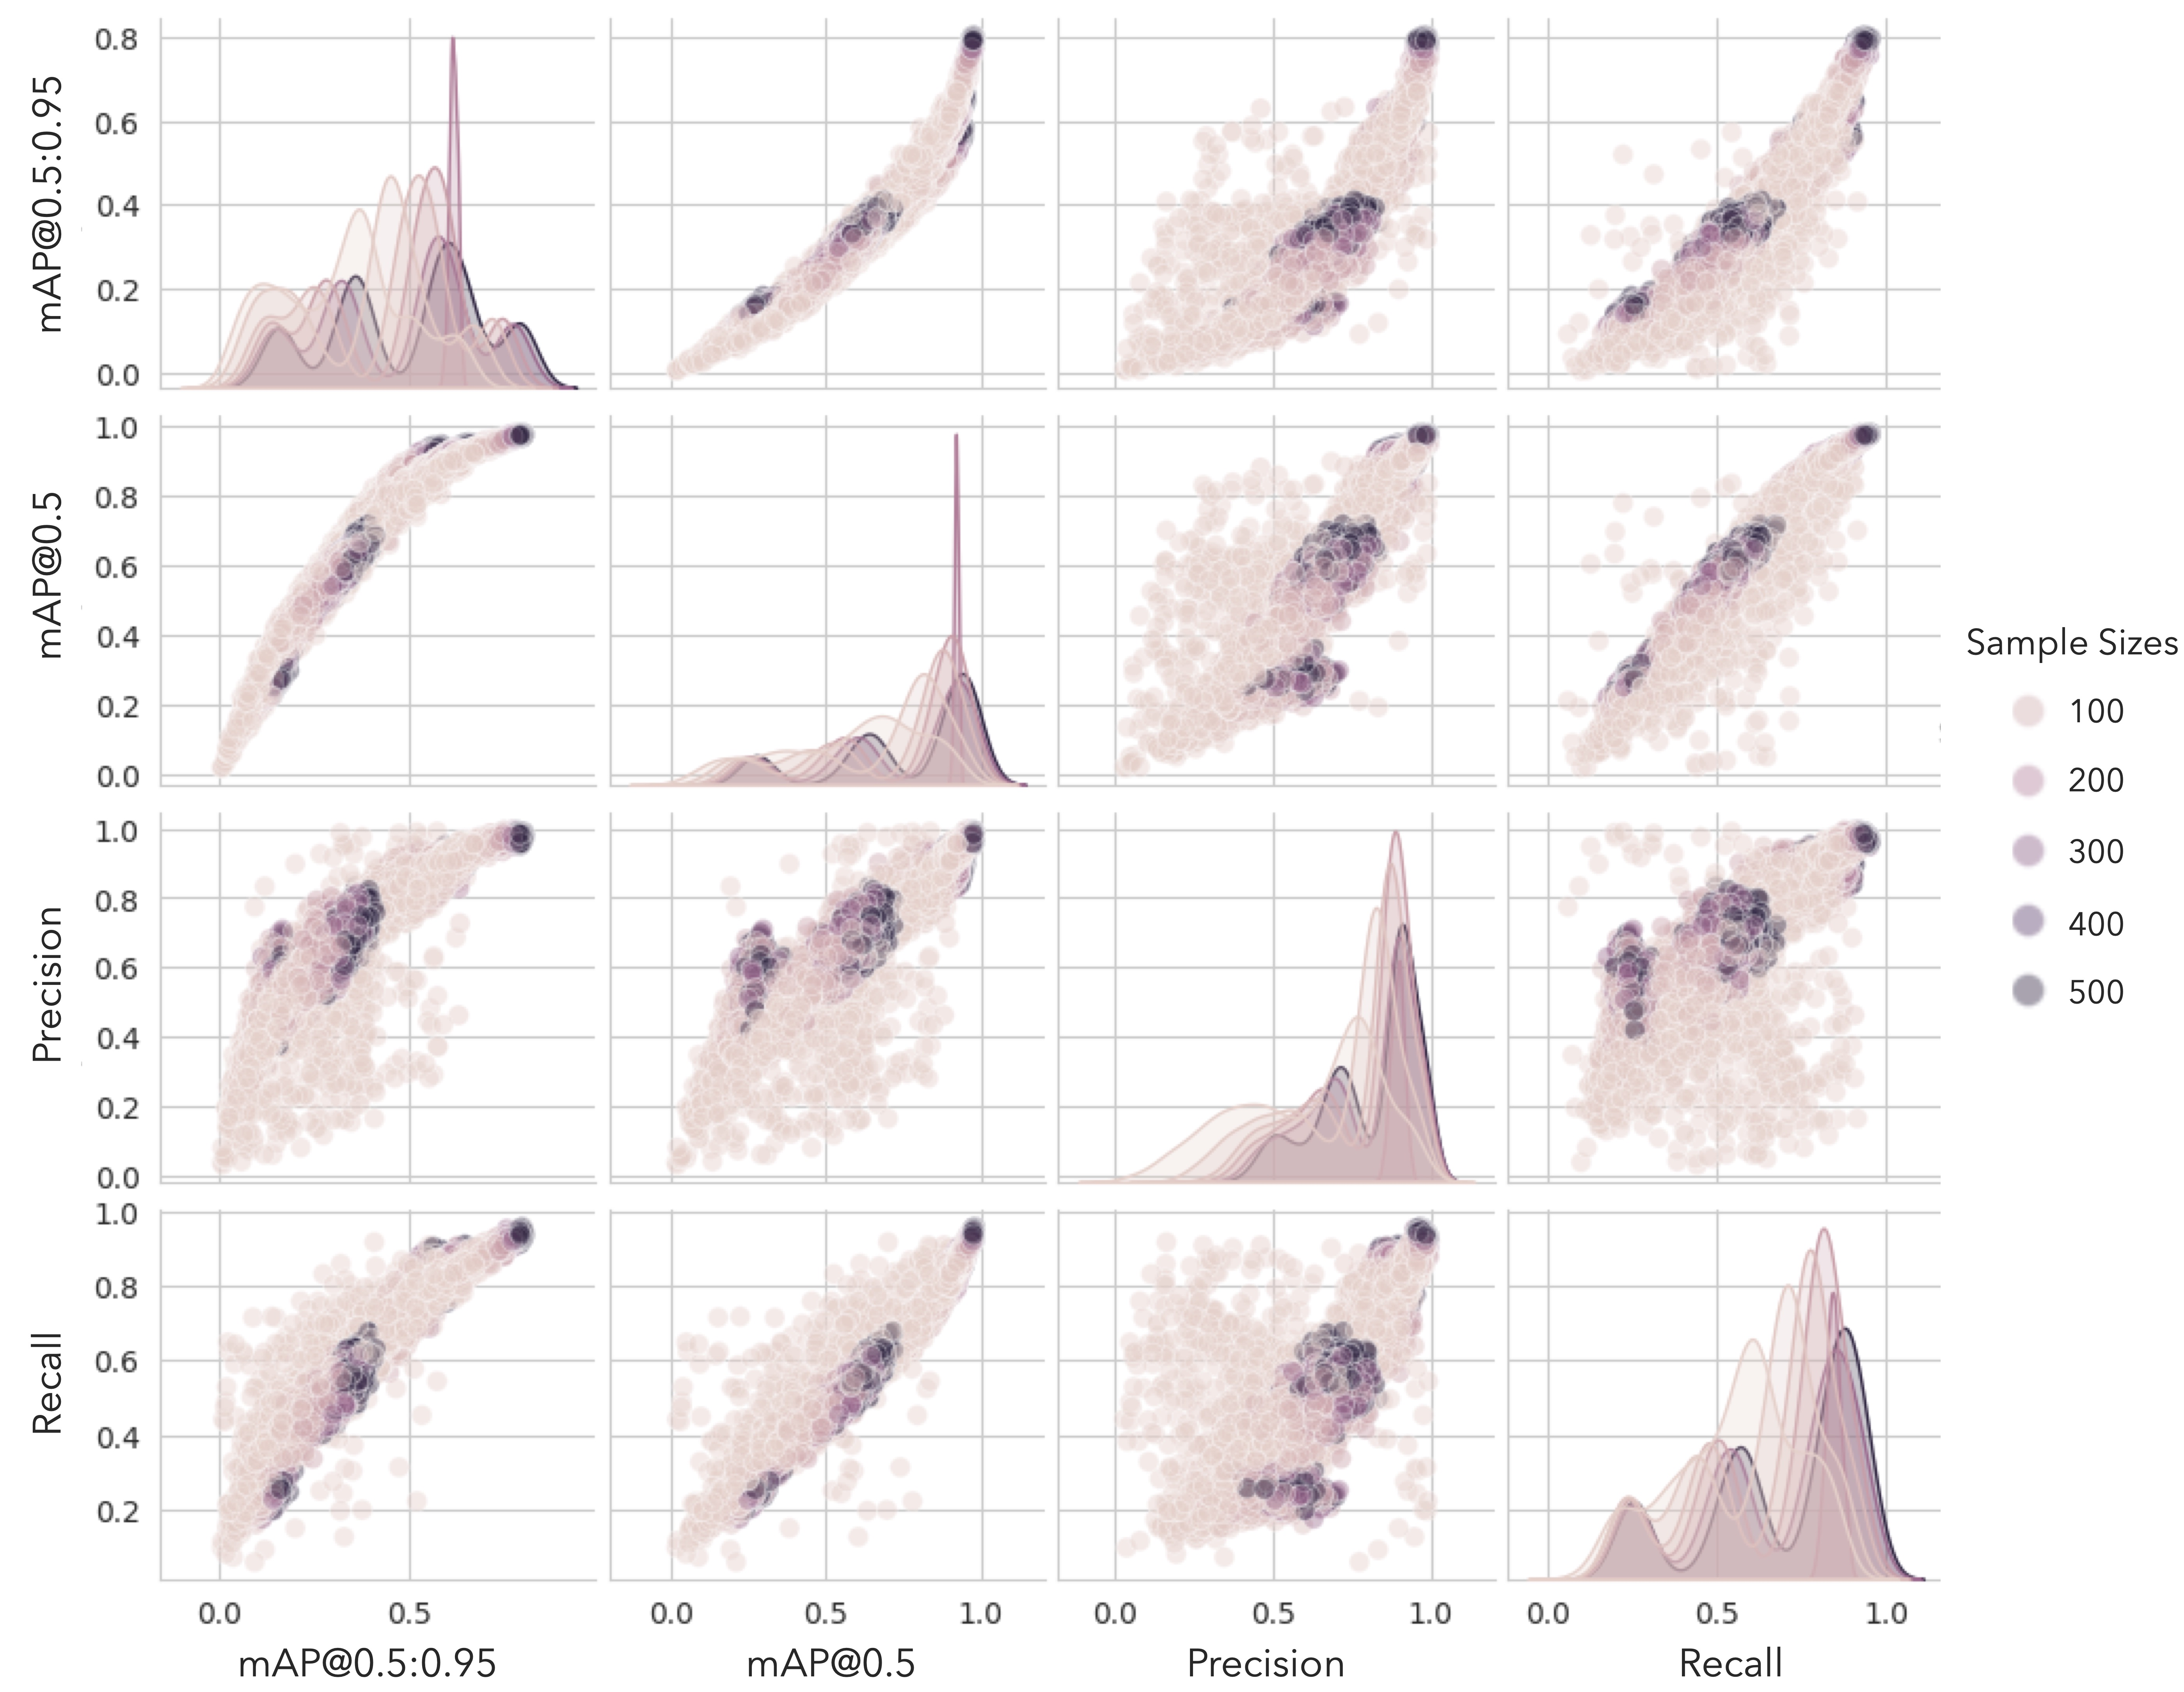
\includegraphics[width=1\textwidth]{Figure/figure_s1.jpg}
    \caption{Example of data annotation }
    \label{fig:metrics}
\end{figure}



\subsection*{Study 1: The changes in camera view angles dramatically affect the model performance}


\begin{figure}[h]
    \centering
    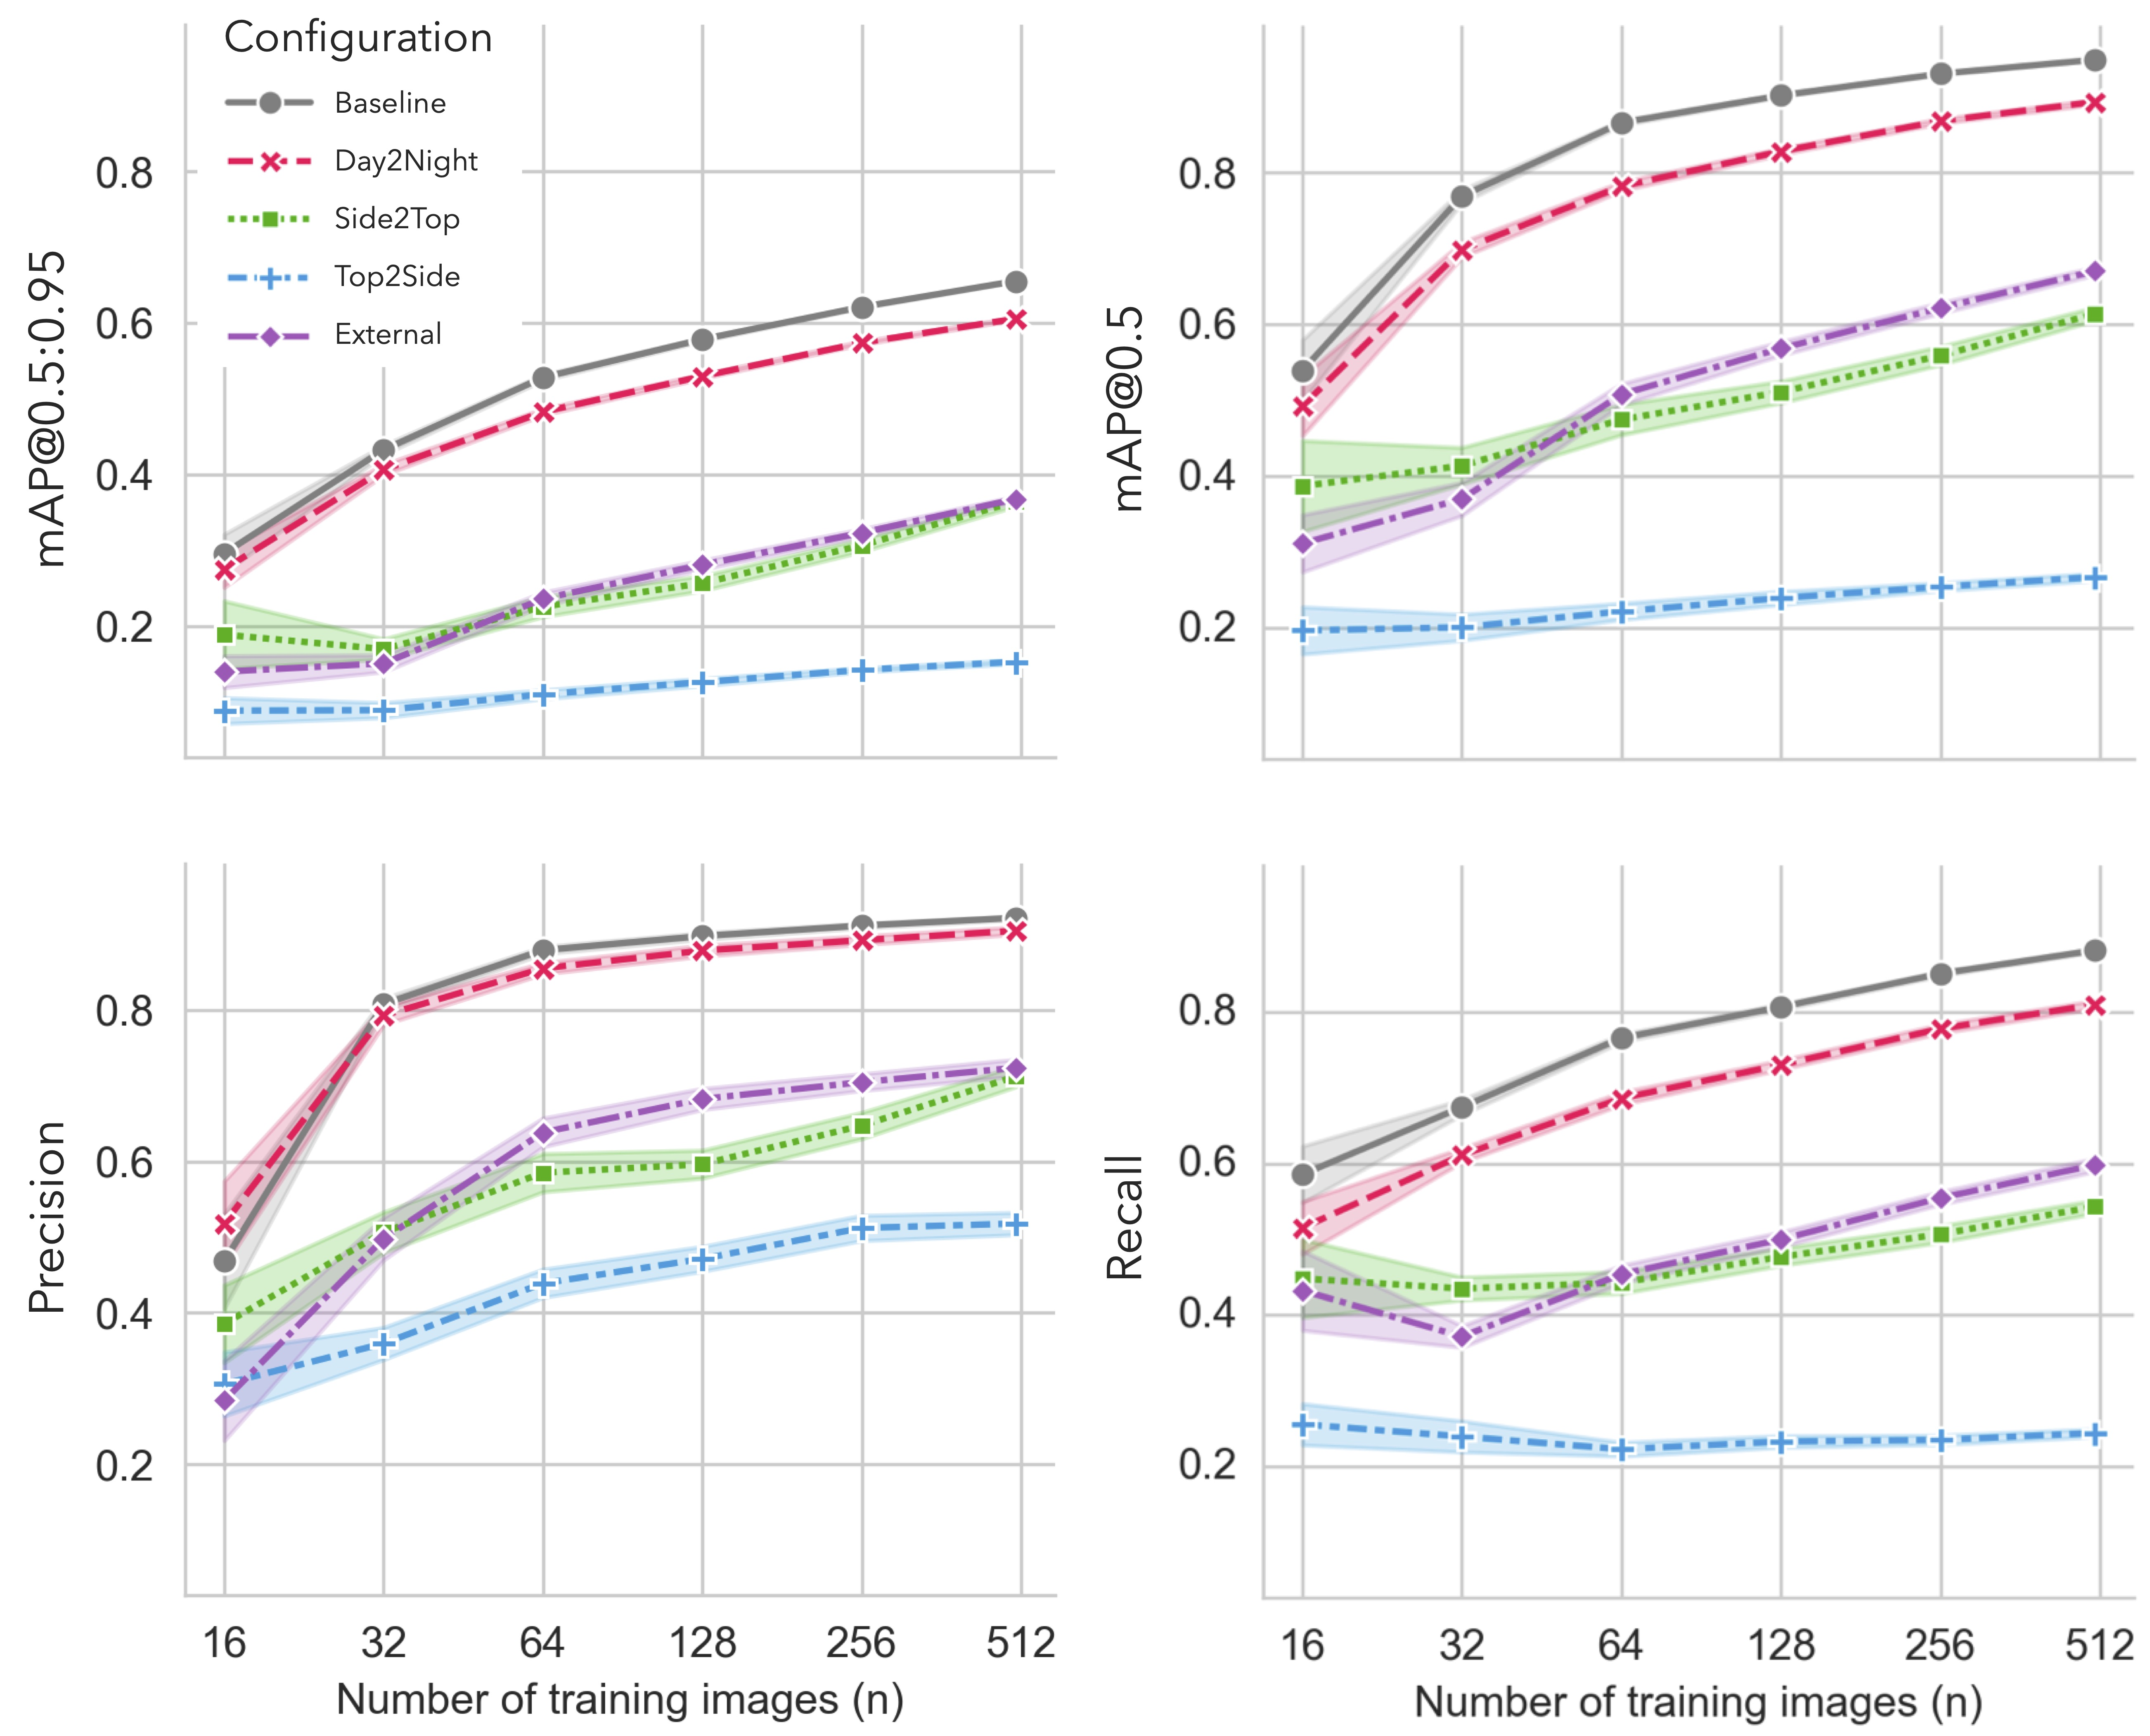
\includegraphics[width=0.8\textwidth]{Figure/figure_3.jpg}
    \caption{The performance of YOLOv9e across various data configurations and training sample sizes. In the upper left and right corners, the plots display the metrics mAP50:95 and mAP50, respectively, for different training samples across diverse data configurations. The lower left and right plots depict precision and recall values, again for varying training samples and configurations.}
    \label{fig:schemes}
    \end{figure}
%The baseline training configuation show a good generalization capabiltiy, in which over 90\% of the predctions were correct in positioning cows at the criteria of 50\% IoU ($\text{mAP@{0.5}}$). Further, the generalization performance can be dissected into changes in view angles (i.e., Top2Side and Side2Top) and lighting condition (i.e., Day2Night). The lightinig condition changes did not dramatically affect the model performance in all four metrics, while changing camera views drop the performance by approxmiately 30\% and 60\% in ($\text{mAP@{0.5}}$ in the configurations of Side2Top and Top2Side, respectively. Across all the metrics and training sample sizes, the configuration of Top2Side consistently showed the worst performance. From the perspective of precision and recall, changing camera from top view to side view result in the model missing detecting more than 7 cows for ever 10 cows and only 50\% of the detection were correct. It is noted that the performance in the Day2Night configuration is closed to the baseline in the metric precision, which only consider predictions with high confidence compared to the metric ($\text{mAP@{0.5}}$). Hence, by excluding the low-confidence predictions, changing ligthing condition did not affect the model performance. Regardless of the configuration and the evaluation metrics, the model performances always increase as the trianing sampel sizes increase.
%%%%%%%%%%%%%%%%% written by me %%%%%%%%%%%%%%%%%%%%%
The baseline training configuration demonstrated a strong generalization capability, with over 90\% of predictions correctly positioning cows at the 50\% IoU criterion ($\text{mAP@{0.5}}$). Further analysis of generalization performance considered changes in view angles (i.e., Top2Side and Side2Top) and lighting conditions (i.e., Day2Night). Changes in lighting conditions did not significantly affect model performance across all four metrics. However, changes in camera views led to performance drops of approximately 30\% and 60\% in $\text{mAP@{0.5}}$ for the Side2Top and Top2Side configurations, respectively. Across all metrics and training sample sizes, the Top2Side configuration consistently showed the worst performance.

From the perspective of precision and recall, changing the camera view from top to side resulted in the model missing more than 7 out of every 10 cows, with only 50\% of detections being correct. Notably, the performance in the Day2Night configuration was close to the baseline in terms of precision, which considers only high-confidence predictions, compared to $\text{mAP@{0.5}}$. This suggests that excluding low-confidence predictions mitigates the impact of lighting changes on model performance. Regardless of configuration and evaluation metrics, model performance consistently improved with increased training sample sizes.

To further illustrate these findings, we observed that while lighting condition changes had minimal impact, the drastic decrease in performance with changing camera angles underscores the importance of viewpoint consistency in training data. For practical applications, this suggests that for environments where camera viewpoints vary significantly, additional training data from multiple angles is essential to maintain high model accuracy. Furthermore, our results highlight that while model complexity can contribute to performance, the quality and diversity of the training dataset play an equally, if not more, critical role. This reinforces the necessity for well-rounded datasets that capture the variability encountered in real-world scenarios to develop robust livestock detection systems.
%\subsection*{Study 2: A higher model complexity does not always lead to better performance}


%\begin{figure}[h]
    %\centering
    %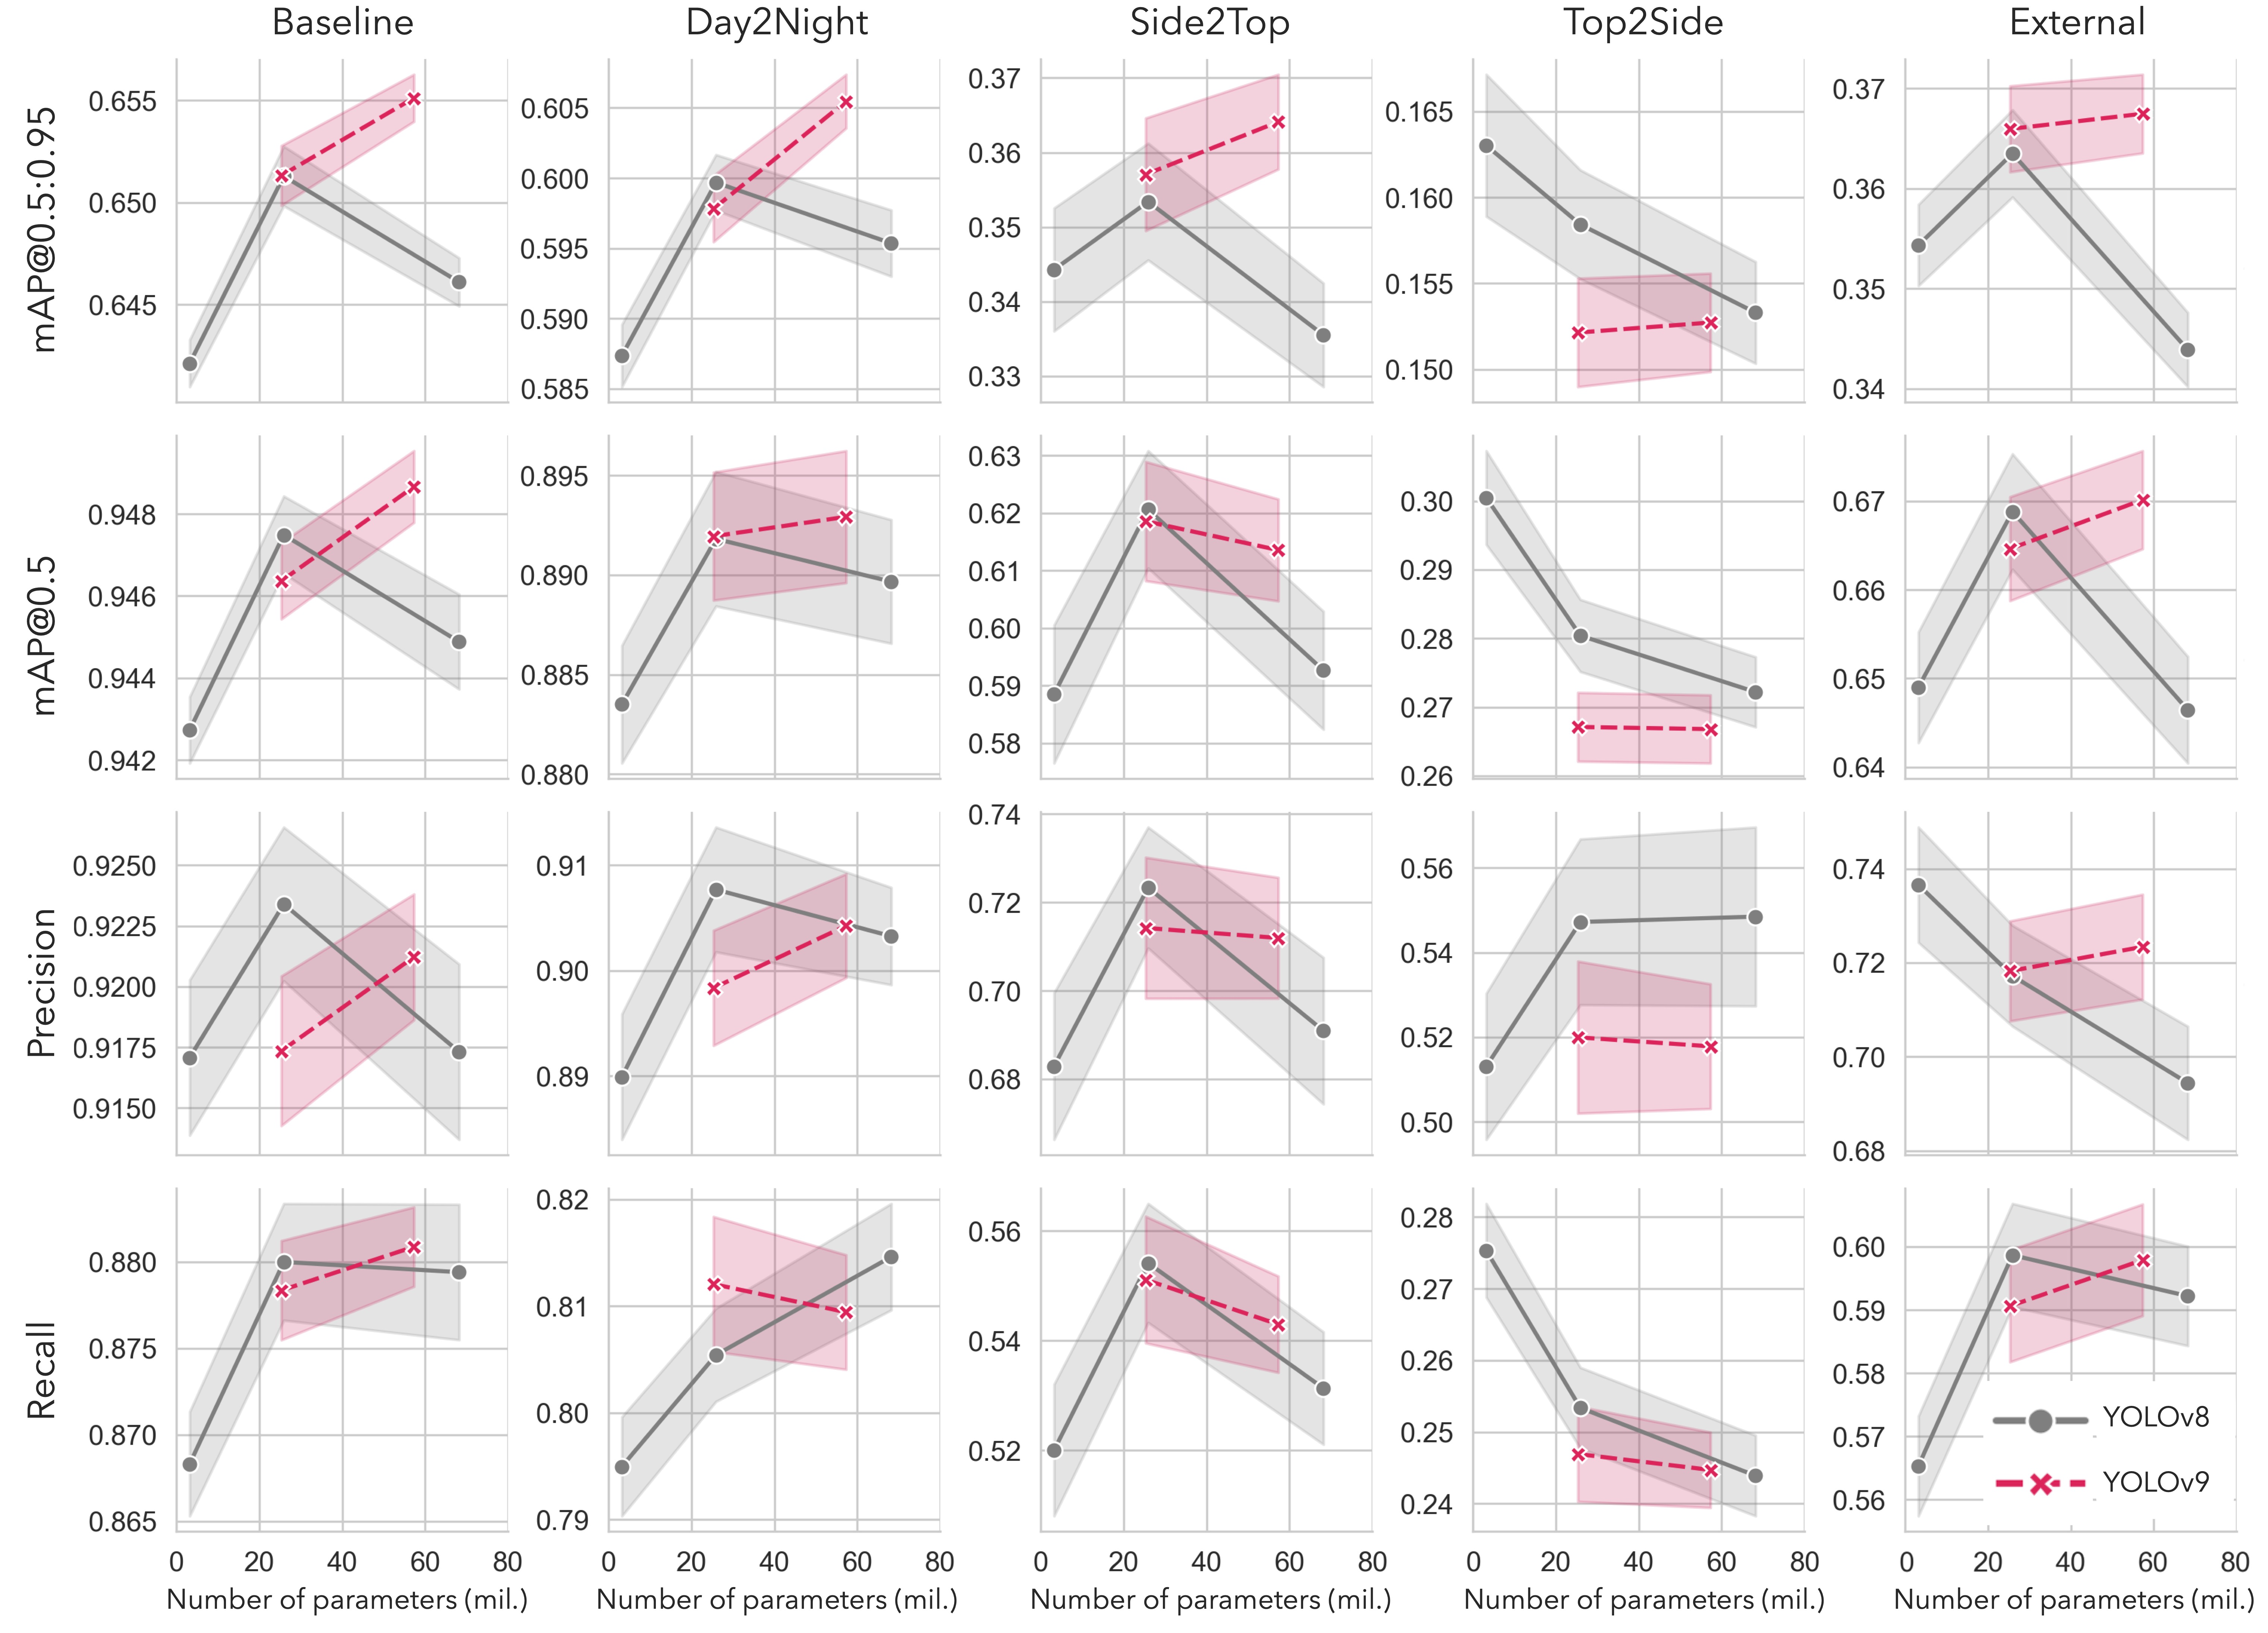
\includegraphics[width=1\textwidth]{Figure/figure_4.jpg}
    %\caption{The performance of YOLOv8 and YOLOv9 models across various model parameters and data configurations, evaluated using four metrics: mAP 50:95, mAP 50, precision, and recall. Each column indicates different data configuration, starting from top to right `Baseline', `Day2Night', `Side2Top' and `Top2Side', `External' respectively. The horizontal axis of all plots indicates the number of model parameter.}
    %\label{fig:models}
%\end{figure}


%From the study, it is found that the xxx of the training configuration affects the relationship between the model complexity and the performance. Based on the study 1, predicting images from the side view based on the model trained on from the top-view camera is the most challenging tasks. In this configuration, increasing the model complexity, except for few cases, the model generalization always became worse than the simple models are. However, in other configurations that show better generalization in the Study 1, the peak performance did not always found from the most complex model. For example, in the baseline, the model that performed that best is YOLOv9e in metrics of $\text{mAP@{0.5:0.95}}$, $\text{mAP@{0.5}}$, and recall. And YOLOv8m performed the best in precision. Neither of the model has the most parameter counts compared to YOLOv8x. It is also worth noting that, different model architecture show different trend in the performance over model complexity. The YOLOv8-family models more likely to have the best performance with the mid-sized model (i.e., YOLOv8m). While in YOLOv9, larger models usually performed better. Hence, the study concluded that the model performacne is determined by both training configuration and the model archtecture.

%The required computational resources can be evaluated from training time (Figure ~\ref{fig:resources}a), inference time (Figure ~\ref{fig:resources}b), adn the memory storage sizes (Figure ~\ref{fig:resources}c). The training time was presented as a ratio of the actual training time over the baseline, which is the time required to train the YOLOv8n model with only 32 samples. The results suggested that using the largest model, YOLOv8x, that with 20 times more parameters, the training time increased by 4 to 6 times based on the training sample size. Additionally, the YOLOv9 models overall required more training time and slower inference frames per seconds (FPS) compared to the YOLOv8 models. The gap of the training time was expanded as the training samples increased. The inference time was calculated as the average FPS in a batch of 64 images. Running the models on CPU with the smallest model (i.e., YOLOv8n), was found to be slower than running the largest model (i.e., YOLOv8x) on GPU, where the FPS were 19.77 and 29.21, respectively. The importance of high FPS models was highlighted in this study, as a real-time inference usually requires a model with FPS higher than 30. Implementing these YOLO models on CPU may not meet this goal according to the result.


%\begin{figure}[h]
   % \centering
    %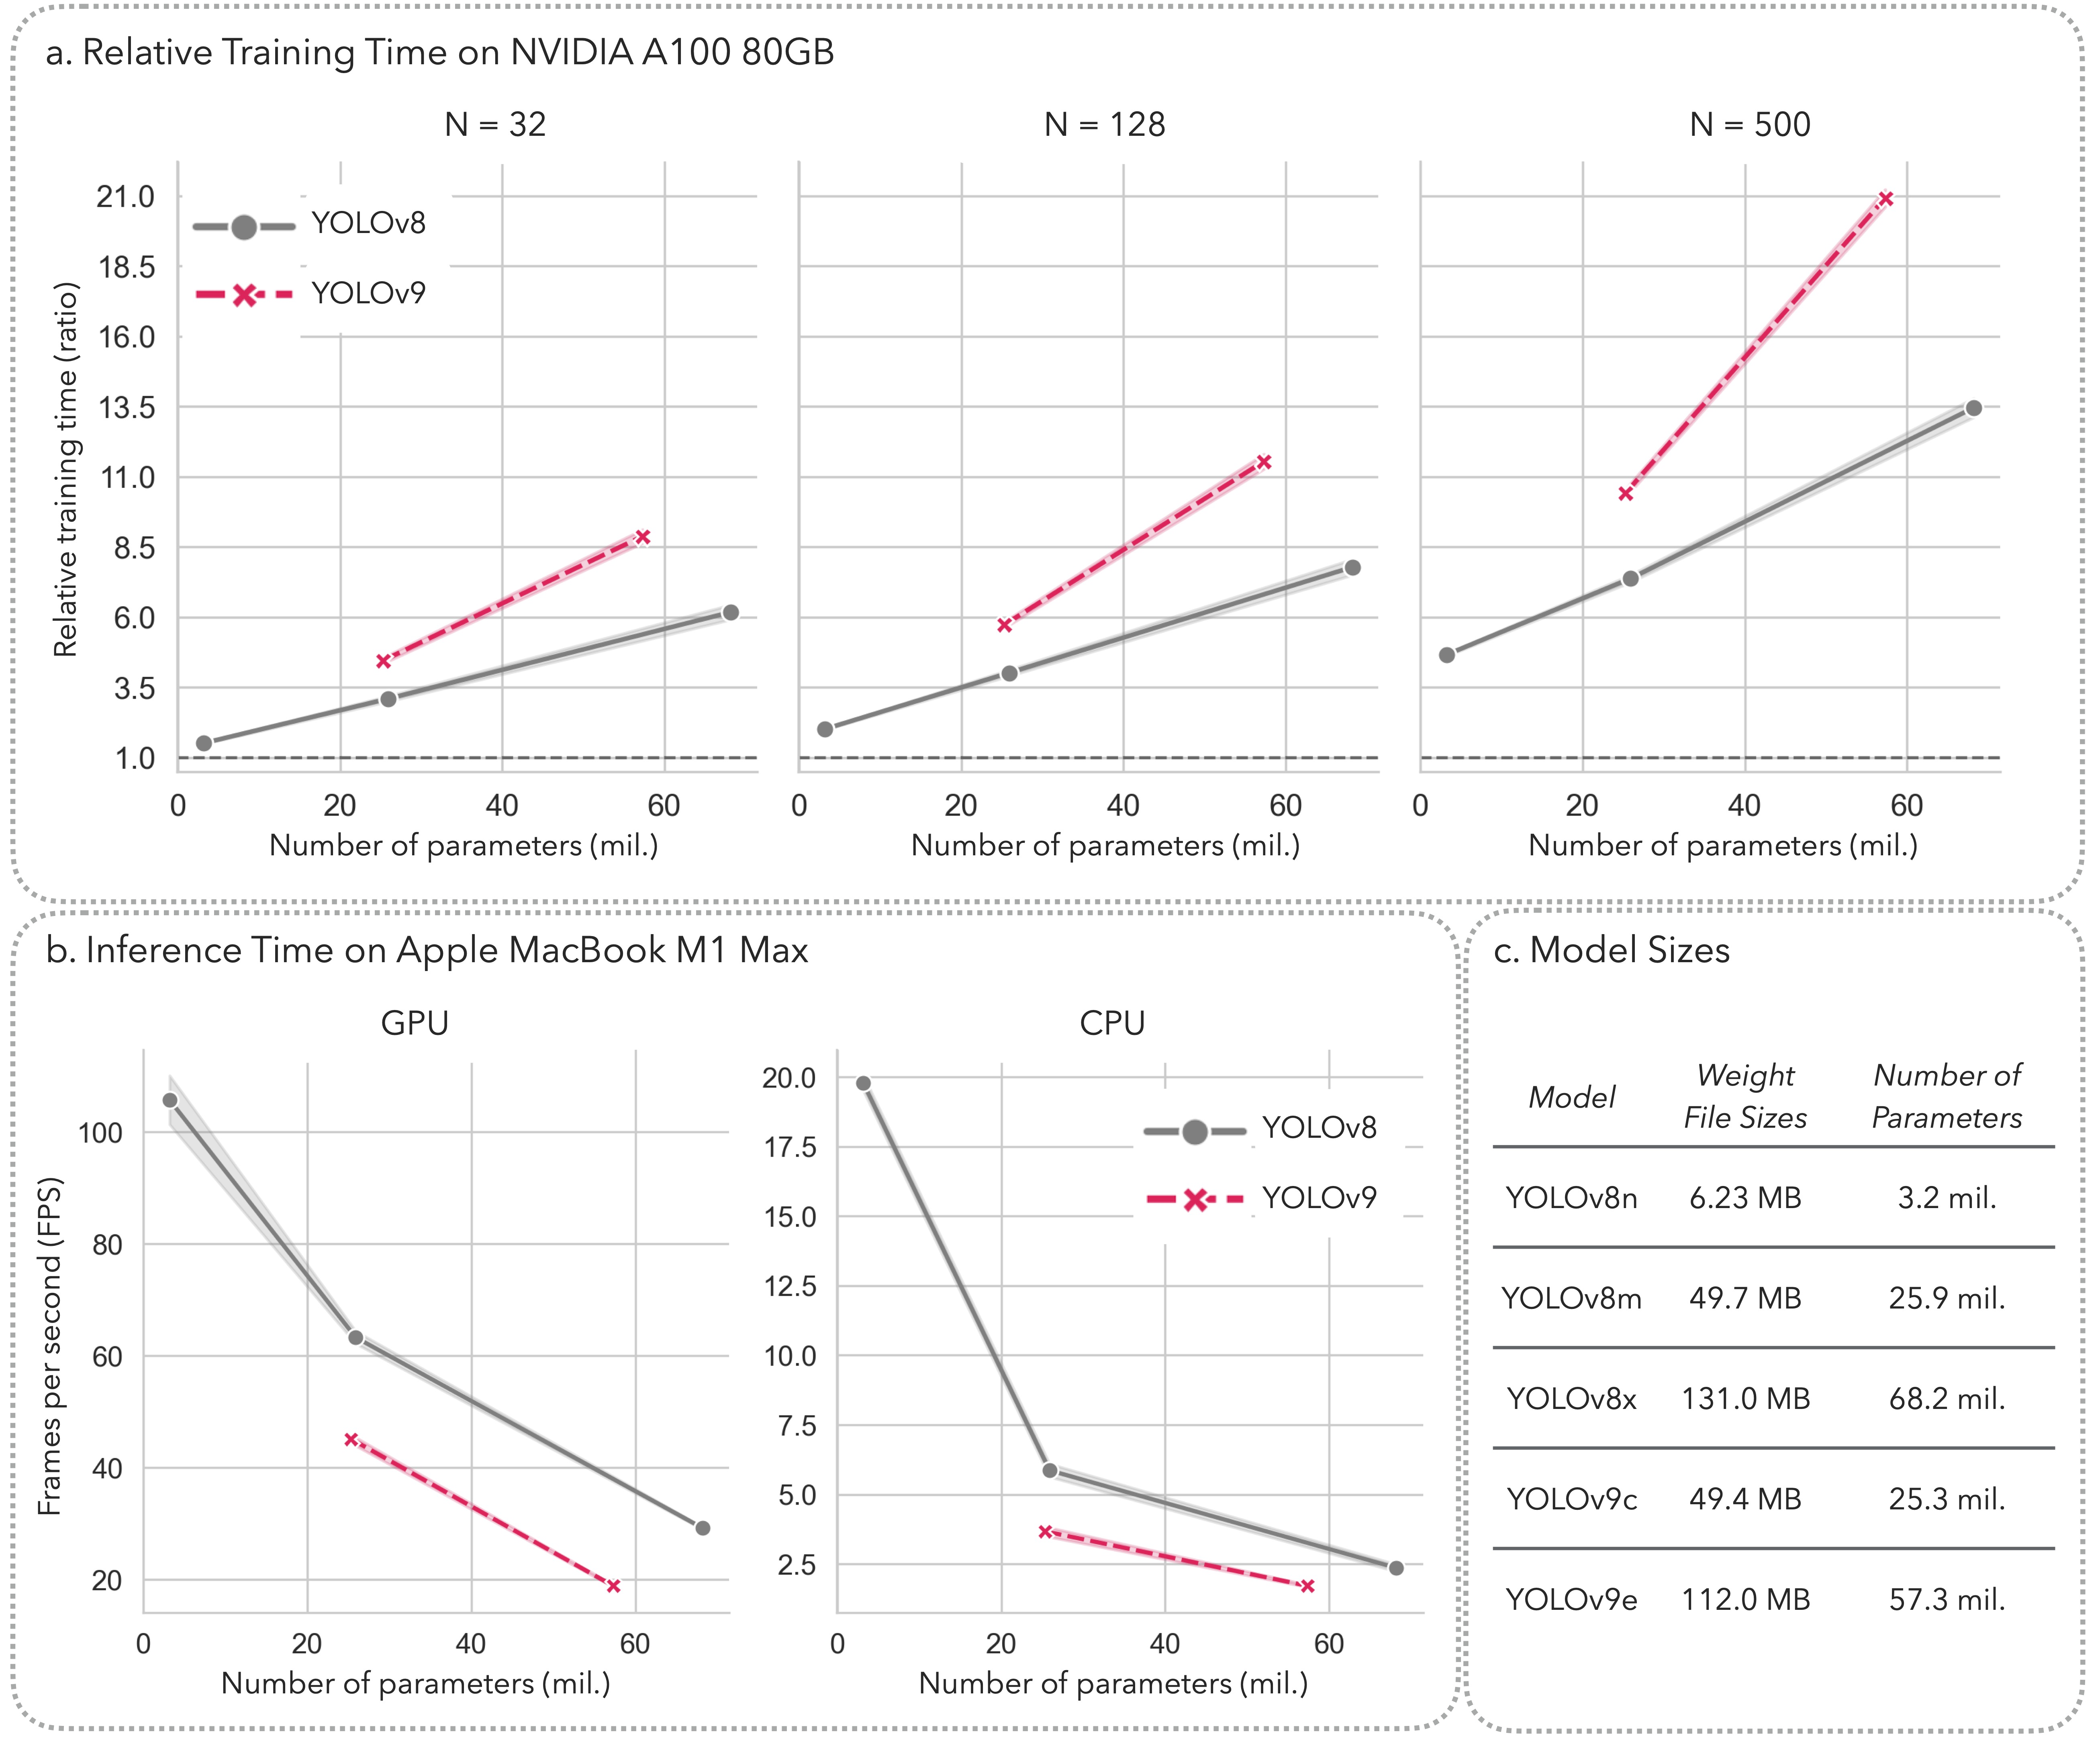
\includegraphics[width=1\textwidth]{figure_6.jpg}
    %\caption{Examples of the annotated images.}
    %\label{fig:resources}
%\end{figure}
%%%%%%%%%%%%%%%%%%%%%%%%%%%%%%%%%%%%%%%%%%%

\subsection*{Study 2: A Higher Model Complexity Does Not Always Lead to Better Performance}

\begin{figure}[h]
\centering
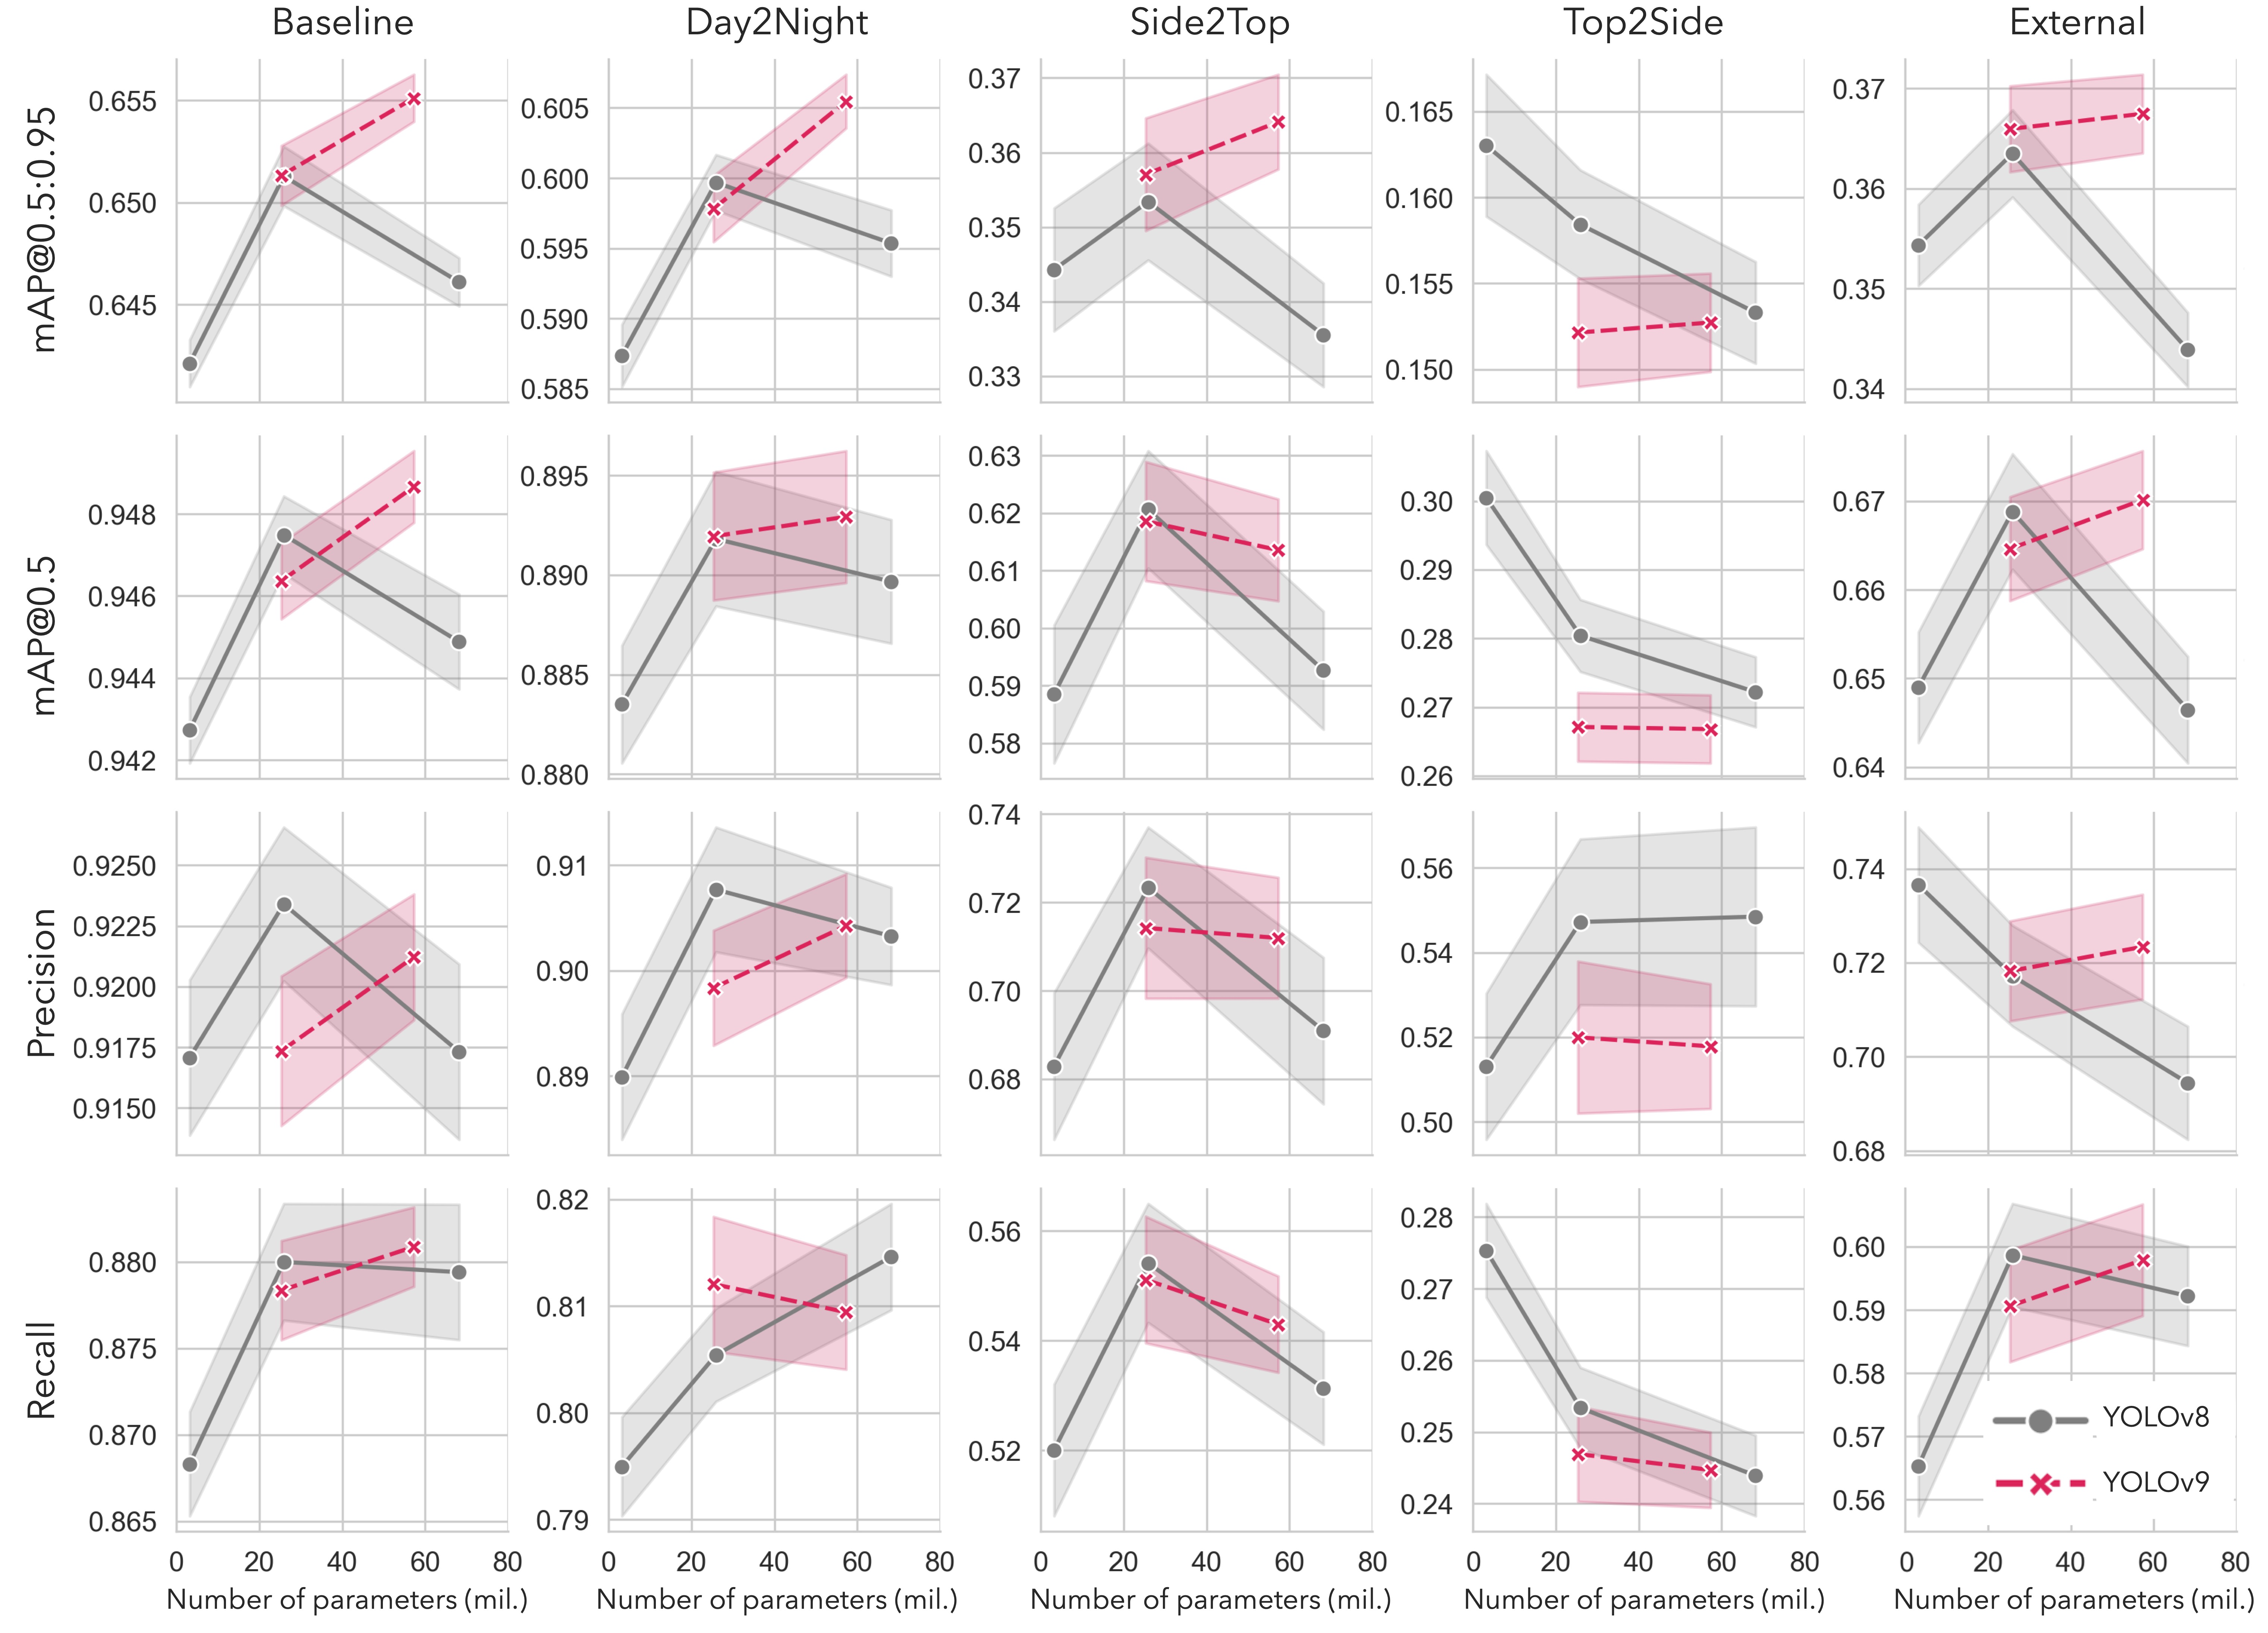
\includegraphics[width=1\textwidth]{Figure/figure_4.jpg}
\caption{The performance of YOLOv8 and YOLOv9 models across various model parameters and data configurations, evaluated using four metrics: mAP 50:95, mAP 50, precision, and recall. Each column indicates a different data configuration, starting from top left to bottom right: Baseline', Day2Night', Side2Top', Top2Side', and `External'. The horizontal axis of all plots indicates the number of model parameters.}
\label{fig:models}
\end{figure}

Our study found that the training configuration significantly affects the relationship between model complexity and performance. Based on Study 1, predicting images from a side view using a model trained on top-view camera images is one of the most challenging tasks. In this configuration, increasing model complexity generally resulted in poorer generalization, with simpler models often performing better. However, in other configurations that demonstrated better generalization in Study 1, the peak performance was not always achieved by the most complex model. For example, in the baseline configuration, the YOLOv9e model performed best in terms of $\text{mAP@{0.5:0.95}}$, $\text{mAP@{0.5}}$, and recall, while the YOLOv8m model excelled in precision. Neither of these models had the highest parameter counts compared to YOLOv8x. It is also worth noting that different model architectures showed different performance trends with varying complexities. The YOLOv8-family models tended to perform best with mid-sized models (i.e., YOLOv8m), whereas larger models in the YOLOv9 family usually performed better. Hence, the study concluded that model performance is determined by both the training configuration and the model architecture.

\begin{figure}[h]
\centering
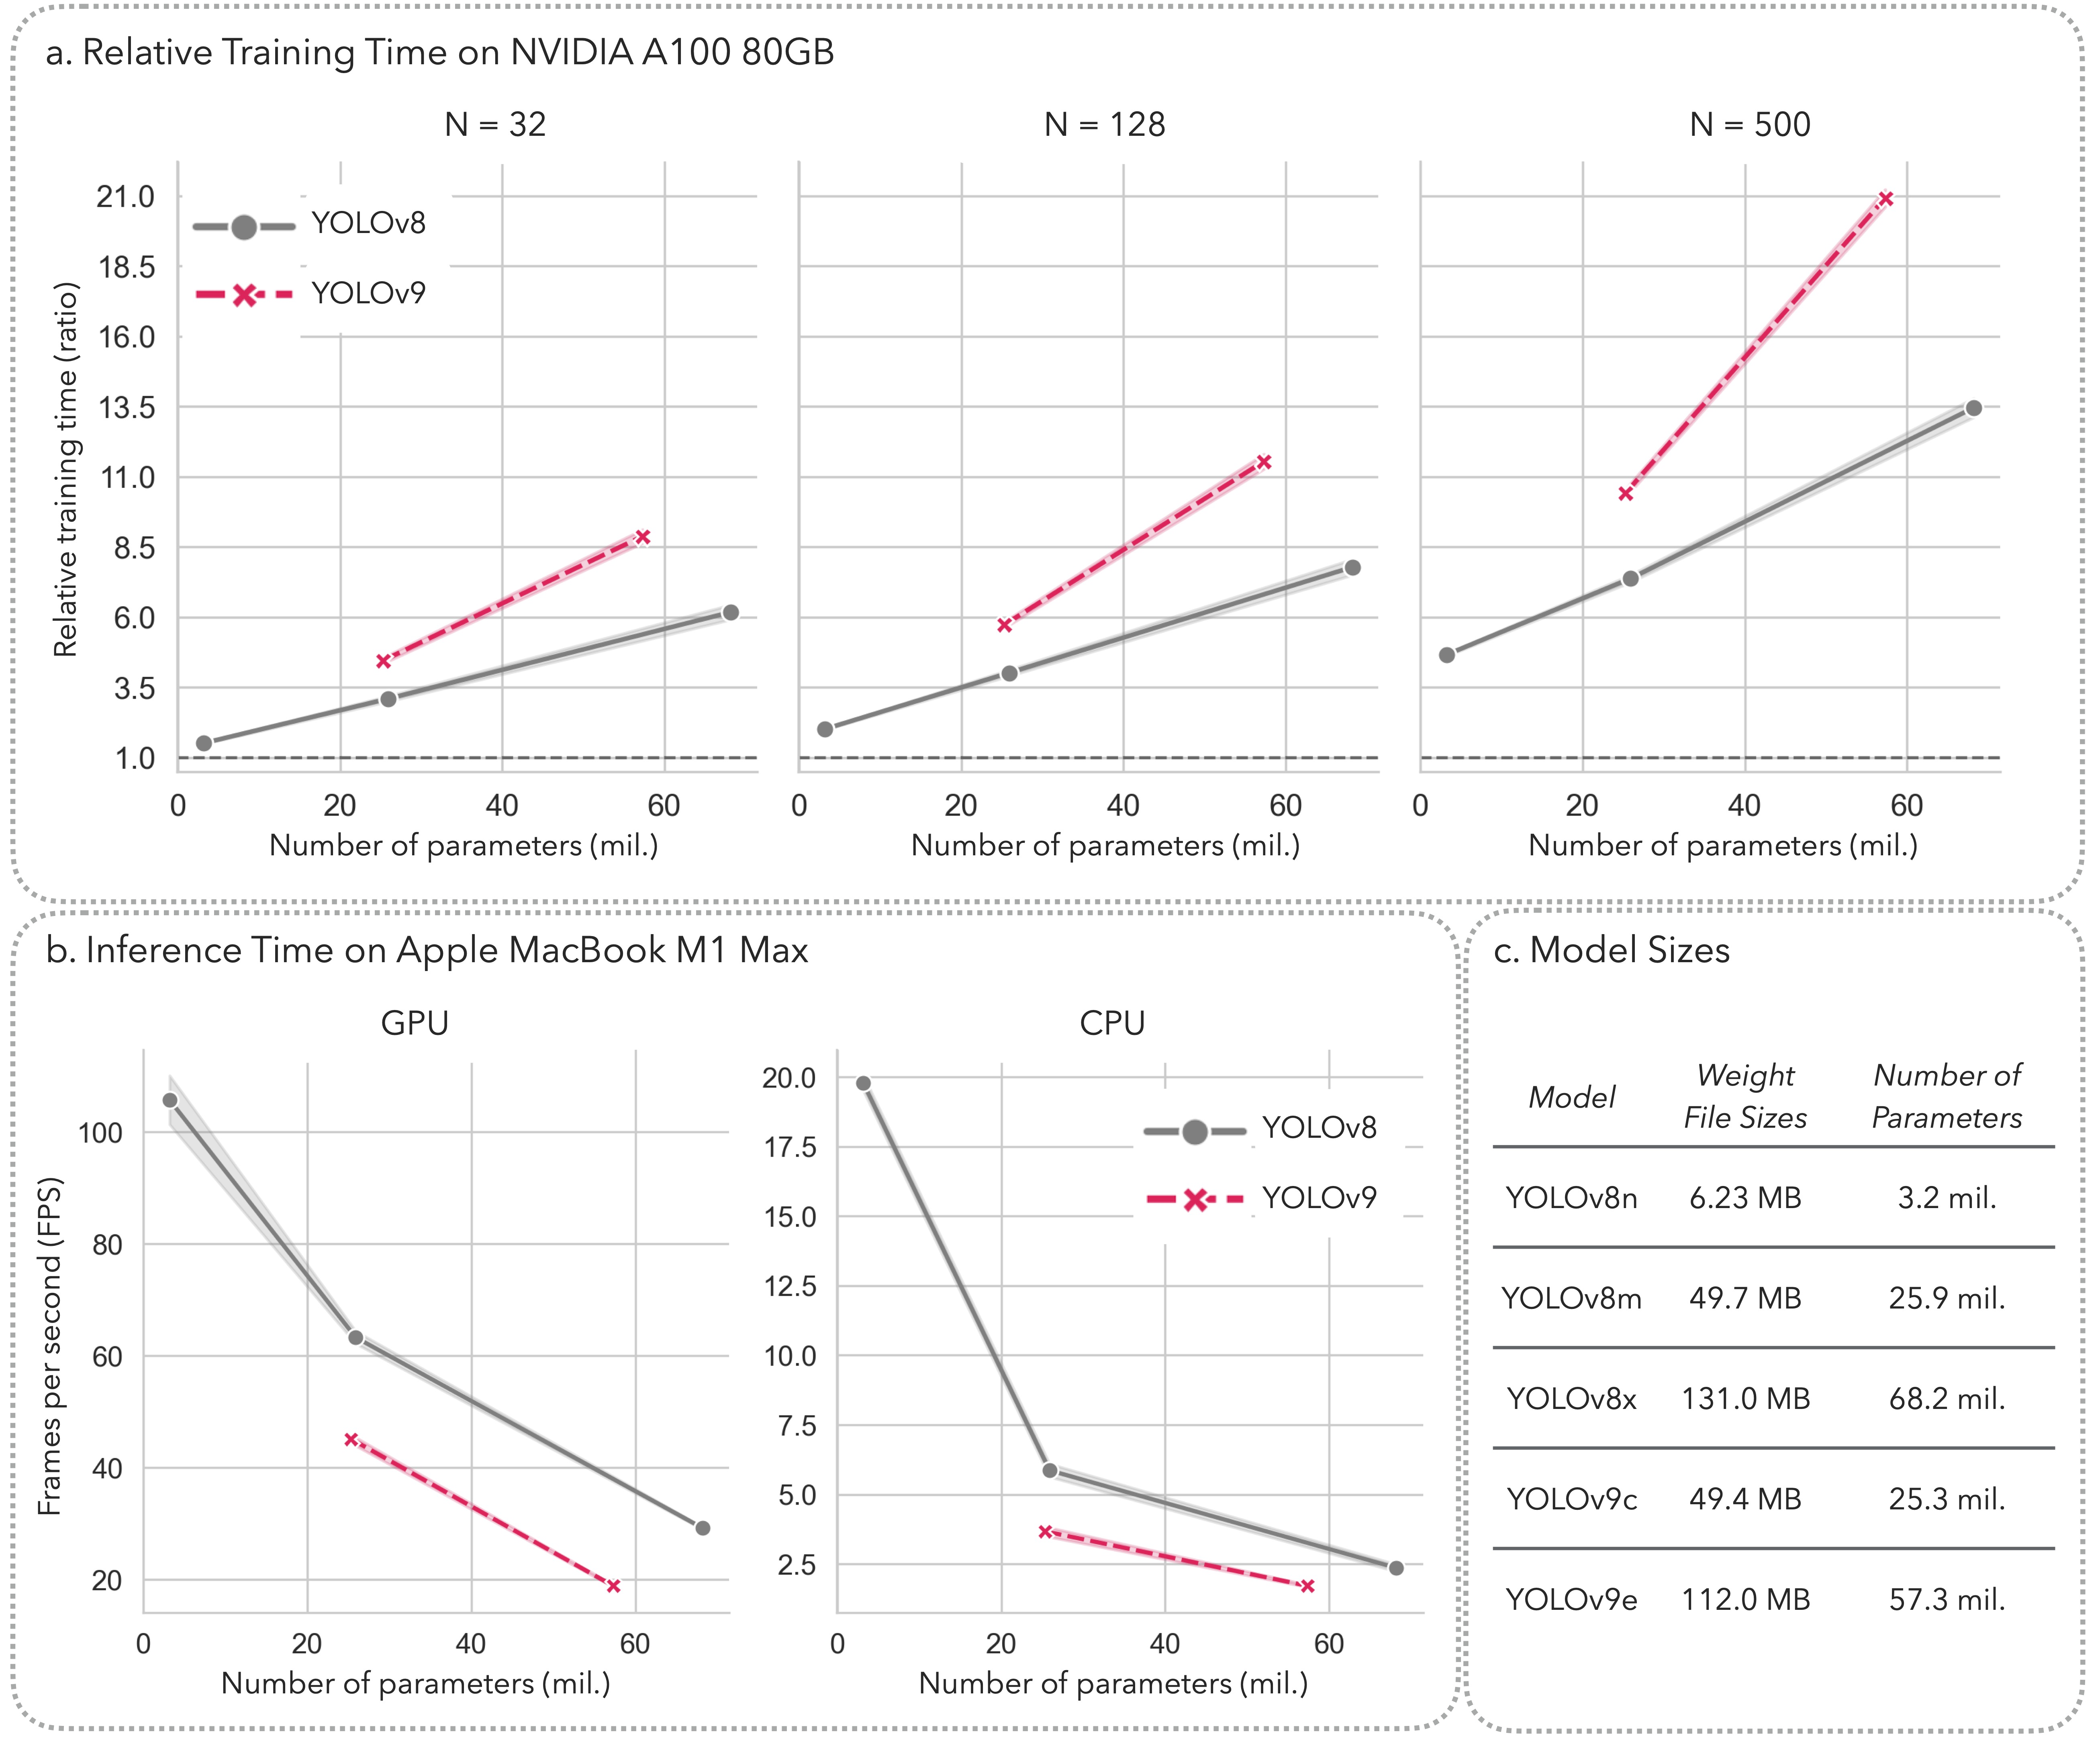
\includegraphics[width=1\textwidth]{figure_6.jpg}
\caption{Examples of the annotated images.}
\label{fig:resources}
\end{figure}


The required computational resources were evaluated in terms of training time (Figure ~\ref{fig:resources}a), inference time (Figure ~\ref{fig:resources}b), and memory storage sizes (Figure ~\ref{fig:resources}c). Training time was presented as a ratio of the actual training time over the baseline, which is the time required to train the YOLOv8n model with only 32 samples. The results suggested that using the largest model, YOLOv8x, with 20 times more parameters, increased training time by 4 to 6 times depending on the training sample size. Additionally, the YOLOv9 models generally required more training time and had slower inference frames per second (FPS) compared to the YOLOv8 models. The gap in training time expanded as the number of training samples increased. Inference time was calculated as the average FPS in a batch of 64 images. Running the models on CPU with the smallest model (i.e., YOLOv8n) was found to be slower than running the largest model (i.e., YOLOv8x) on GPU, where the FPS were 19.77 and 29.21, respectively. The importance of high FPS models was highlighted in this study, as real-time inference usually requires a model with an FPS higher than 30. Implementing these YOLO models on CPU may not meet this requirement according to the results.



%%%%%%%%%%%%%%%%%%%%%%%%%%%%%%%%%%%%%%%%%%%

\subsection*{Study 3: The advantages of fine-tuning the model is limited when the model is simple}

%The results presented in Figure \ref{fig:finetune} indicate that the benefit of using fine-tuned initial weights is minimal for simpler models. Specifically, when employing YOLOv8n, the performance difference between the default and fine-tuned weights was insignificant when fine-tuning data from the Top-View Camera and Side-View Camera. However, as the model complexity increased, a greater number of fine-tuning samples were required for the two different initial weights to achieve similar performance. For instance, in the case of YOLOv9e, the performance gap was eliminated when the number of fine-tuning samples reached 128 and 64 for the Top-View Camera and Side-View Camera data sources, respectively. The similar trend was observed from the External camera, where a significant performance gap of more than 25\% in mAP50:95 was observed for YOLOv9e when the sample size was 16. It is also noted that, although the performance gap was closed to zero from the Top-View Camera and Side-View Camera data sources, the gap was never closed for the External camera. In summary, using fine-tuned initial weights is only beneficial for models with larger parameter sizes (e.g., YOLOv8x, YOLOv9c, and YOLOv9e) and when limited training samples are available.
The results presented in Figure \ref{fig:finetune} indicate that the benefit of using fine-tuned initial weights is minimal for simpler models. Specifically, when employing YOLOv8n, the performance difference between the default and fine-tuned weights was insignificant when fine-tuning data from the Top-View Camera and Side-View Camera. However, as model complexity increased, a greater number of fine-tuning samples were required for the two different initial weights to achieve similar performance. For instance, in the case of YOLOv9e, the performance gap was eliminated when the number of fine-tuning samples reached 128 and 64 for the Top-View Camera and Side-View Camera data sources, respectively. A similar trend was observed with the External camera, where a significant performance gap of more than 25\% in $\text{mAP@{0.5:0.95}}$ was observed for YOLOv9e when the sample size was 16. It is also noted that, although the performance gap was closed to zero for the Top-View Camera and Side-View Camera data sources, the gap was never closed for the External camera. In summary, using fine-tuned initial weights is only beneficial for models with larger parameter sizes (e.g., YOLOv8x, YOLOv9c, and YOLOv9e) and when limited training samples are available.

\begin{figure}[h]
    \centering
    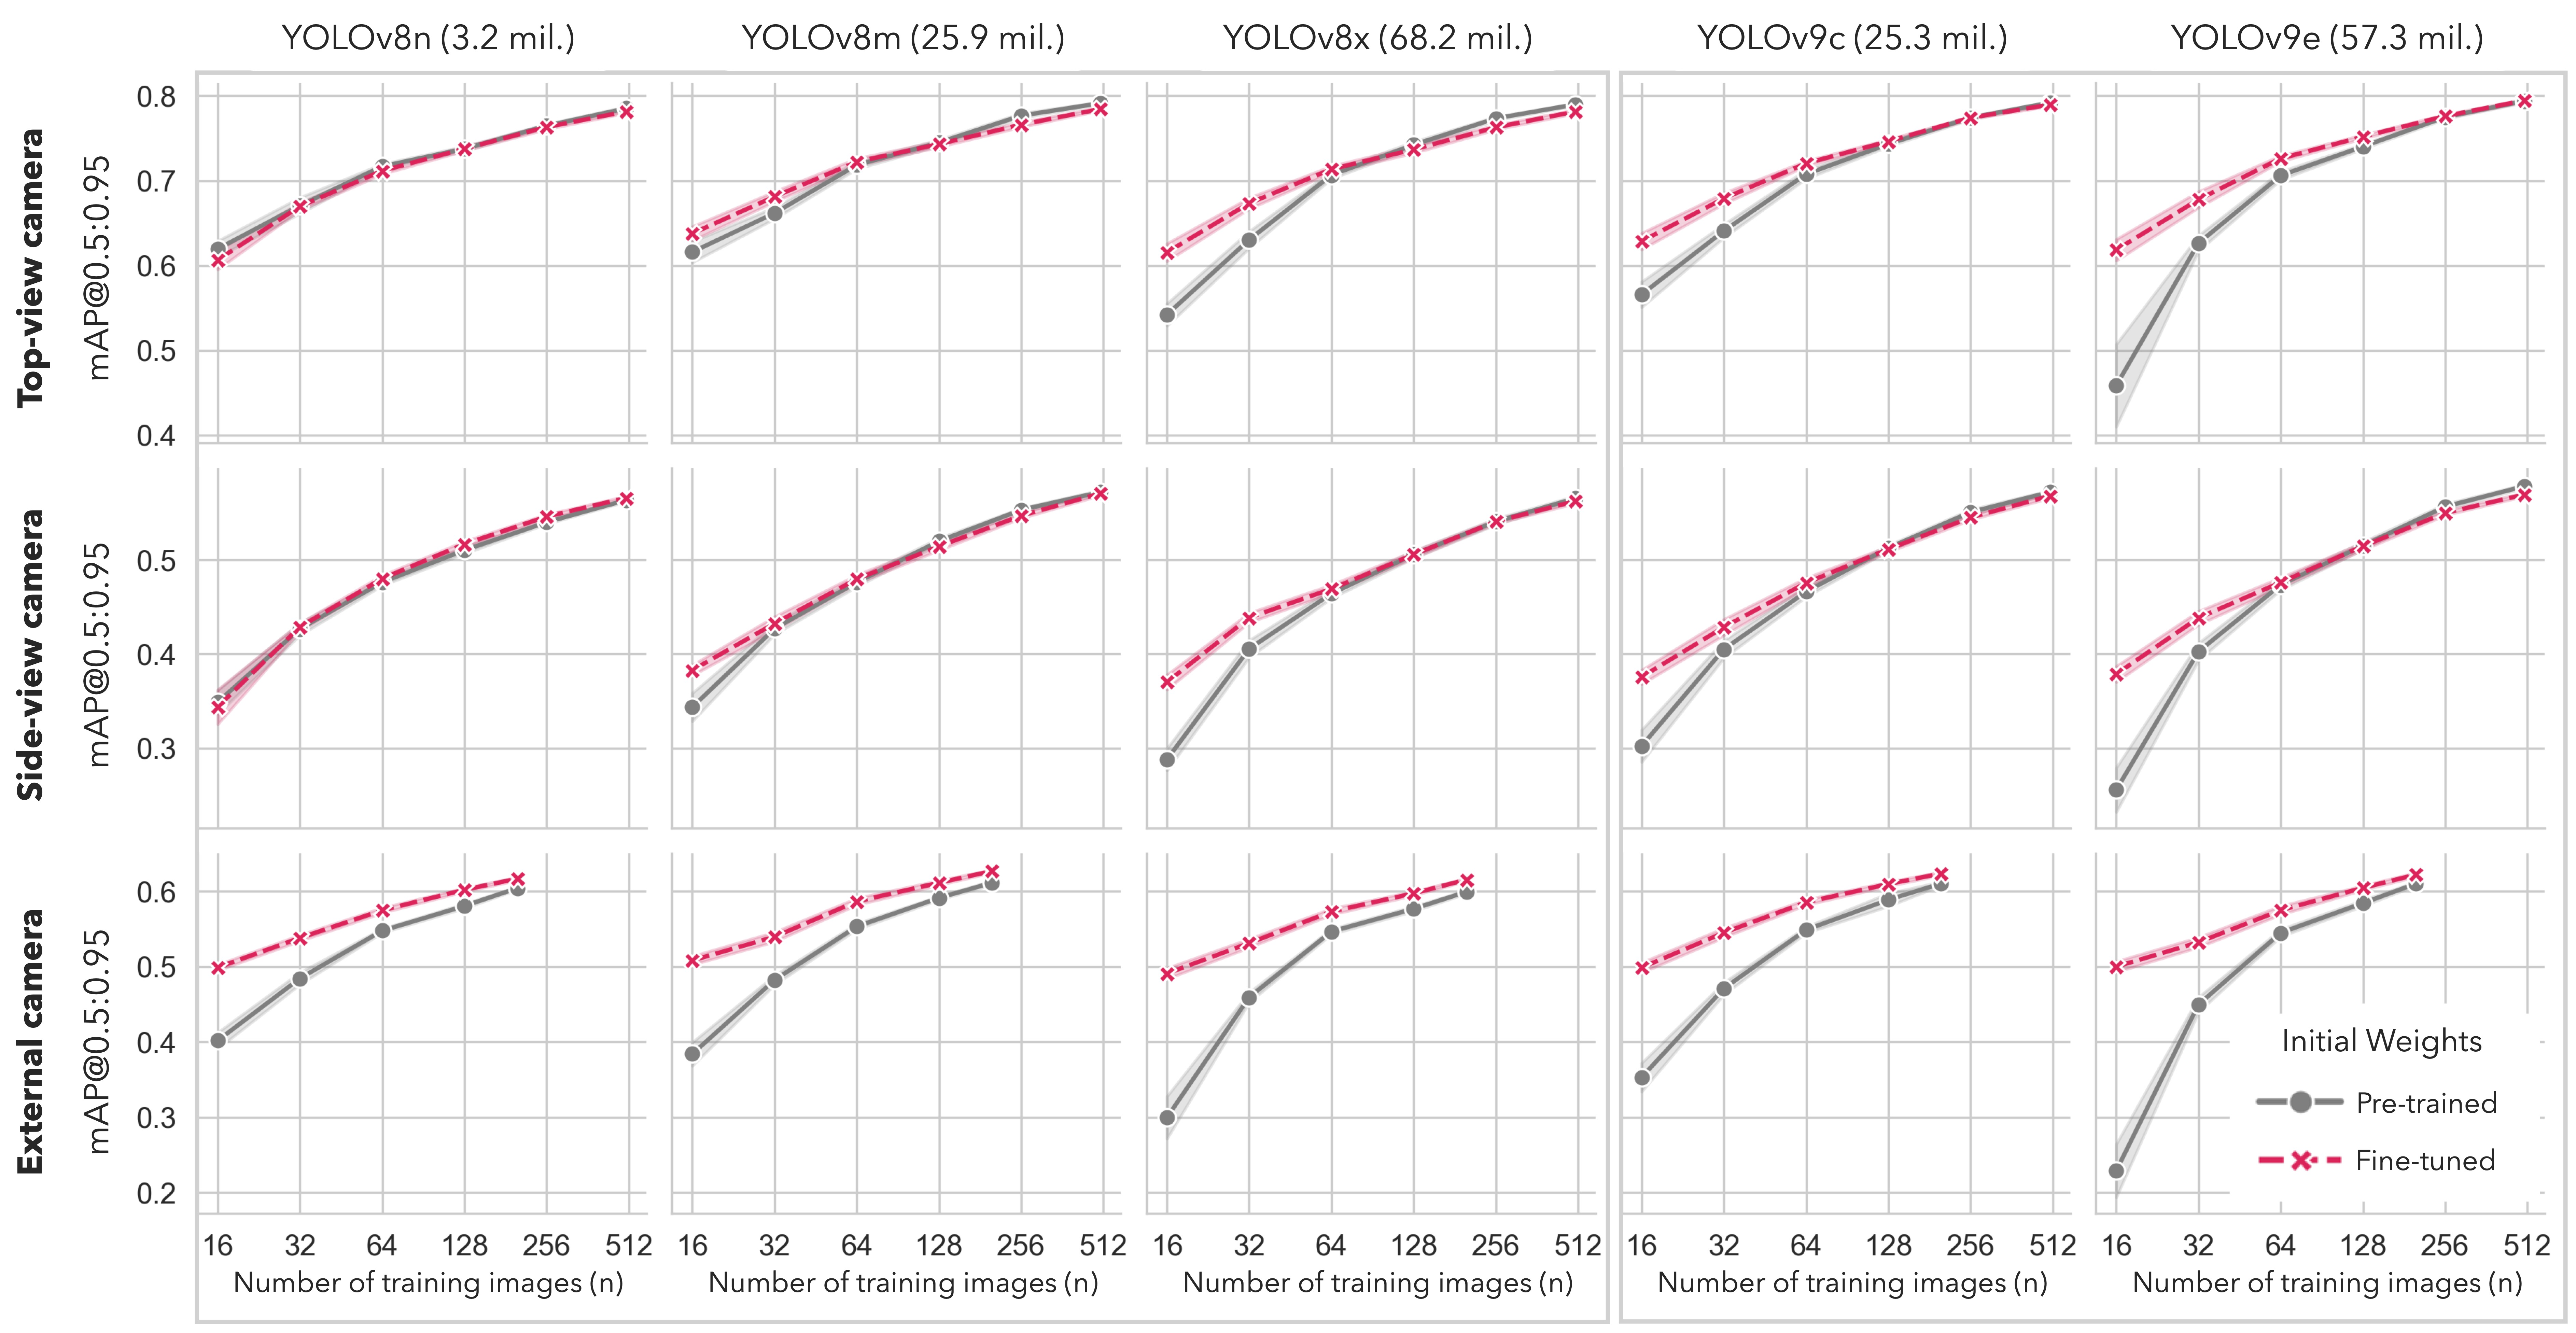
\includegraphics[width=1\textwidth]{Figure/figure_5.jpg}
    \caption{Variation in mAP50:95 across different models, sample sizes, and weight initialization conditions. Green lines represent instances where weights were initialized with fine-tuned models (cases 3 and 4, as detailed in Table ~\ref{tab:configuration}), while orange lines indicate scenarios employing default weights (trained with the COCO dataset). The horizontal axis indicates the number of training samples used for fine-tuning.}
    \label{fig:finetune}
\end{figure}



\subsubsection*{Discussion for Study 1: Potential causes for the performance drop in camera view points}

Figure ~\ref{fig:schemes} provides a comparative analysis of model behavior under various data configurations. It is clear that the `Day2Night' configuration shown a much better performance relative to the heterogeneous viewpoint-oriented configurations `Top2Side' and `Side2Top'.

Despite the various challenges in adapting models from day to night conditions, the `Day2Night' configuration consistently maintains high precision, closely mirroring the `Baseline' configuration across all training sample sizes. This suggests that changes in lighting have less impact on the models ability to detect objects compared to changes in viewpoint. This robustness to lighting could be attributed to the inclusion of diverse lighting conditions in the training phase, specifically, model performance benefited from pixel-wise augmentation techniques such as adjustments to hue, saturation, and value(HSV). These augmentations introduced a variety of color variations to the images, enhancing the model's ability to generalize across different visual conditions.Such methods adjust the lighting and contrast in training images, enhancing the model's ability to generalize to different illumination scenarios. Moreover, these YOLO models benefit from pre-training on the COCO dataset, which is characterized by a wide array of images with varied lighting, aiding their adaptability to shifts in light.

On the other hand, the models perform sub optimally in scenarios involving changes in viewpoint. This is because each new viewpoint can introduce fundamentally different object features, which are not replicated through standard data augmentation methods like lighting or affine transformations. For example, when the camera was placed at a lower angle, cows were occluded more by stalls and fences. These additional objects posed object-wise variation that can not be overcome by augmentation of HSV space or image translation.

The analysis of Figure ~\ref{fig:finetune} provides another insight on the performance across homogeneous viewpoint data configurations, specifically `Top-view camera' and `Side-view camera'. The data demonstrates that the `Top-view camera' configuration consistently yields higher mAP values regardless of the training sample size and weight initialization conditions. This implies that the `Side-view camera' configuration, where both training and test images are captured from the side view, presents a more formidable challenge for cow detection compared to the `Top-view camera' configuration.

Similarly to the discussion of the difference between lighting and viewpoint in the images, the side view poses difficulties due to occlusions by neighboring cows and additional distractions, such as obstacles in aisles and fences. Furthermore, cows located further away in side-view images may not be as visible, complicating feature extraction. In contrast, the `Top-view camera' configuration benefits from an unobstructed aerial perspective, ensuring that the top view of all cow instances is clearly visible and free from such obstructions. This distinction in visibility between the two configurations contributes to the ease of feature extraction and ultimately, the performance disparity observed.

\subsubsection*{Discussion for Study 2: The Choice of Model Complexity is Task-Specific}

The results from Figure \ref{fig:models} show the relationship between the number of model parameters and object detection performance across various data configurations for YOLOv8 and YOLOv9 models.

When trained on the COCO dataset \cite{lin2014microsoft}, both YOLOv8 \cite{ultralyticsYOLOv8} and YOLOv9 \cite{wang2024yolov9} models exhibit an increase in $\text{mAP@{0.5}}$ as the number of parameters increases. The rate of performance increase demonstrates a concave upward trajectory in the curve plotting mAP against the number of parameters. Despite this observation, the data from Figure \ref{fig:models} do not support a definitive conclusion that a higher number of parameters consistently enhances model performance. For all data configurations analyzed, performance changes minimally with parameter variations and does not adhere to a consistent pattern.

Within the YOLOv8 series, the YOLOv8m model delivers optimal performance across almost all data configurations, except for Top2Side'. In this particular configuration, there is a gradual decline in performance as the number of parameters increases. On the other hand, the YOLOv9 series shows a slight improvement in performance for the all configurations except the camera viewpoint configurations. For Top2Side, YOLOv9 consistently performs the worst, even with the complex models. Also, from Study 1, we observed that Top2Side` is considered the most difficult task among all datasets. This outcome might suggest that when the task is too difficult, the superior capability of the model may no longer hold in such cases. In general, the performance trends of these models with respect to parameter increments are not uniform; in some cases, there is a slight enhancement, whereas in others, a small reduction in performance is noted.

The prior work's findings were based on the COCO dataset, which encompasses 80 classes and predominantly features standalone images. In contrast, our study utilizes an indoor farm dataset focused exclusively on a single class: cows. Consequently, the model may not require as many parameters to optimally discern the necessary features for cow detection. This reminds researchers to not solely rely on a model known for its best performance on a public dataset. The generalization performance may be case-specific.


\subsubsection*{Discussion of Study 3: The custom weight initialization is beneficial for model fine-tuning only if the  model is complex and the data is limitated}

In our study goal 3, we examine the impact of different weight initialization strategies on the fine-tuning of models, as detailed in Figure \ref{fig:finetune}. Our findings indicate that for YOLO models with fewer parameters, such as YOLOv8n and YOLOv8m, the choice of weight initialization does not make a significant difference in fine-tuning performance. In contrast, larger models like YOLOv8x, YOLOv9c, and YOLOv9e exhibit improved performance when weights are initialized from a model that has been previously fine-tuned, as highlighted in cases 2 and 4 in Table \ref{tab:configuration}.

Therefore, when fine-tuning larger models with a limited dataset, it is beneficial to utilize weights previously fine-tuned on various data configurations. This approach leverages the additional learned features and adaptability from the initial fine-tuning, resulting in better performance even with a small amount of new data. For example, our results showed that YOLOv9e achieved optimal performance with fewer fine-tuning samples when initialized with fine-tuned weights compared to default weights.

Conversely, for smaller models, the weight initialization strategy does not significantly impact fine-tuning performance. This is likely due to the lower complexity and fewer parameters of these models, which makes them less dependent on the initial weight configuration to achieve good performance. In practical terms, this means that for simpler models, researchers can save time and computational resources by directly fine-tuning without the need for customized weight initialization.

In summary, the study underscores the importance of custom weight initialization for fine-tuning larger models, especially when dealing with limited data. Utilizing fine-tuned weights can substantially enhance model performance, making it a crucial consideration in the deployment of complex models in resource-constrained environments. Conversely, simpler models do not benefit as much from this strategy, allowing for more straightforward and efficient fine-tuning processes.







